\documentclass[a4paper]{book}
\usepackage{a4wide}
\usepackage{makeidx}
\usepackage{graphicx}
\usepackage{multicol}
\usepackage{float}
\usepackage{listings}
\usepackage{color}
\usepackage{textcomp}
\usepackage{alltt}
\usepackage{times}
\usepackage{ifpdf}
\ifpdf
\usepackage[pdftex,
            pagebackref=true,
            colorlinks=true,
            linkcolor=blue,
            unicode
           ]{hyperref}
\else
\usepackage[ps2pdf,
            pagebackref=true,
            colorlinks=true,
            linkcolor=blue,
            unicode
           ]{hyperref}
\usepackage{pspicture}
\fi
\usepackage[utf8]{inputenc}
\usepackage{doxygen}
\lstset{language=C++,inputencoding=utf8,basicstyle=\footnotesize,breaklines=true,breakatwhitespace=true,tabsize=8,numbers=left }
\makeindex
\setcounter{tocdepth}{3}
\renewcommand{\footrulewidth}{0.4pt}
\begin{document}
\hypersetup{pageanchor=false}
\begin{titlepage}
\vspace*{7cm}
\begin{center}
{\Large wGui }\\
\vspace*{1cm}
{\large Generated by Doxygen 1.7.1}\\
\vspace*{0.5cm}
{\small Thu Feb 17 2011 09:01:30}\\
\end{center}
\end{titlepage}
\clearemptydoublepage
\pagenumbering{roman}
\tableofcontents
\clearemptydoublepage
\pagenumbering{arabic}
\hypersetup{pageanchor=true}
\chapter{Class Index}
\section{Class Hierarchy}
This inheritance list is sorted roughly, but not completely, alphabetically:\begin{DoxyCompactList}
\item \contentsline{section}{clsContext}{\pageref{classclsContext}}{}
\item \contentsline{section}{clsEventHandlers}{\pageref{classclsEventHandlers}}{}
\item \contentsline{section}{clsFunctions}{\pageref{classclsFunctions}}{}
\item \contentsline{section}{clsPage}{\pageref{classclsPage}}{}
\item \contentsline{section}{clsRequests}{\pageref{classclsRequests}}{}
\item \contentsline{section}{clsValidator}{\pageref{classclsValidator}}{}
\item \contentsline{section}{myExternalClass}{\pageref{classmyExternalClass}}{}
\item \contentsline{section}{myObjectTest}{\pageref{classmyObjectTest}}{}
\item \contentsline{section}{myPreObject}{\pageref{classmyPreObject}}{}
\item \contentsline{section}{objectMethodsTest}{\pageref{classobjectMethodsTest}}{}
\begin{DoxyCompactList}
\item \contentsline{section}{objectMethodsTest2}{\pageref{classobjectMethodsTest2}}{}
\end{DoxyCompactList}
\item \contentsline{section}{xajax}{\pageref{classxajax}}{}
\begin{DoxyCompactList}
\item \contentsline{section}{legacyXajax}{\pageref{classlegacyXajax}}{}
\end{DoxyCompactList}
\item \contentsline{section}{xajaxArgumentManager}{\pageref{classxajaxArgumentManager}}{}
\item \contentsline{section}{xajaxCall}{\pageref{classxajaxCall}}{}
\item \contentsline{section}{xajaxCallableObject}{\pageref{classxajaxCallableObject}}{}
\item \contentsline{section}{xajaxControl}{\pageref{classxajaxControl}}{}
\begin{DoxyCompactList}
\item \contentsline{section}{clsArea}{\pageref{classclsArea}}{}
\item \contentsline{section}{clsBase}{\pageref{classclsBase}}{}
\item \contentsline{section}{clsBr}{\pageref{classclsBr}}{}
\item \contentsline{section}{clsCol}{\pageref{classclsCol}}{}
\item \contentsline{section}{clsFrame}{\pageref{classclsFrame}}{}
\item \contentsline{section}{clsHr}{\pageref{classclsHr}}{}
\item \contentsline{section}{clsImg}{\pageref{classclsImg}}{}
\item \contentsline{section}{clsInput}{\pageref{classclsInput}}{}
\begin{DoxyCompactList}
\item \contentsline{section}{clsInputWithLabel}{\pageref{classclsInputWithLabel}}{}
\end{DoxyCompactList}
\item \contentsline{section}{clsLink}{\pageref{classclsLink}}{}
\item \contentsline{section}{clsLiteral}{\pageref{classclsLiteral}}{}
\item \contentsline{section}{clsMeta}{\pageref{classclsMeta}}{}
\item \contentsline{section}{clsMutuallyExclusiveButton}{\pageref{classclsMutuallyExclusiveButton}}{}
\item \contentsline{section}{clsParam}{\pageref{classclsParam}}{}
\item \contentsline{section}{xajaxControlContainer}{\pageref{classxajaxControlContainer}}{}
\begin{DoxyCompactList}
\item \contentsline{section}{clsAnchor}{\pageref{classclsAnchor}}{}
\item \contentsline{section}{clsBody}{\pageref{classclsBody}}{}
\item \contentsline{section}{clsButton}{\pageref{classclsButton}}{}
\item \contentsline{section}{clsCaption}{\pageref{classclsCaption}}{}
\item \contentsline{section}{clsColgroup}{\pageref{classclsColgroup}}{}
\item \contentsline{section}{clsDd}{\pageref{classclsDd}}{}
\item \contentsline{section}{clsDiv}{\pageref{classclsDiv}}{}
\item \contentsline{section}{clsDl}{\pageref{classclsDl}}{}
\item \contentsline{section}{clsDoctype}{\pageref{classclsDoctype}}{}
\item \contentsline{section}{clsDocument}{\pageref{classclsDocument}}{}
\item \contentsline{section}{clsDt}{\pageref{classclsDt}}{}
\item \contentsline{section}{clsFieldset}{\pageref{classclsFieldset}}{}
\item \contentsline{section}{clsForm}{\pageref{classclsForm}}{}
\item \contentsline{section}{clsFrameset}{\pageref{classclsFrameset}}{}
\item \contentsline{section}{clsHead}{\pageref{classclsHead}}{}
\item \contentsline{section}{clsHeadline}{\pageref{classclsHeadline}}{}
\item \contentsline{section}{clsHtml}{\pageref{classclsHtml}}{}
\item \contentsline{section}{clsIframe}{\pageref{classclsIframe}}{}
\item \contentsline{section}{clsInlineContainer}{\pageref{classclsInlineContainer}}{}
\begin{DoxyCompactList}
\item \contentsline{section}{clsAbbr}{\pageref{classclsAbbr}}{}
\item \contentsline{section}{clsAcronym}{\pageref{classclsAcronym}}{}
\item \contentsline{section}{clsAddress}{\pageref{classclsAddress}}{}
\item \contentsline{section}{clsBig}{\pageref{classclsBig}}{}
\item \contentsline{section}{clsBlockquote}{\pageref{classclsBlockquote}}{}
\item \contentsline{section}{clsBold}{\pageref{classclsBold}}{}
\item \contentsline{section}{clsCite}{\pageref{classclsCite}}{}
\item \contentsline{section}{clsCode}{\pageref{classclsCode}}{}
\item \contentsline{section}{clsDel}{\pageref{classclsDel}}{}
\item \contentsline{section}{clsDfn}{\pageref{classclsDfn}}{}
\item \contentsline{section}{clsEm}{\pageref{classclsEm}}{}
\item \contentsline{section}{clsIns}{\pageref{classclsIns}}{}
\item \contentsline{section}{clsItalic}{\pageref{classclsItalic}}{}
\item \contentsline{section}{clsKbd}{\pageref{classclsKbd}}{}
\item \contentsline{section}{clsParagraph}{\pageref{classclsParagraph}}{}
\item \contentsline{section}{clsPre}{\pageref{classclsPre}}{}
\item \contentsline{section}{clsSamp}{\pageref{classclsSamp}}{}
\item \contentsline{section}{clsSmall}{\pageref{classclsSmall}}{}
\item \contentsline{section}{clsStrong}{\pageref{classclsStrong}}{}
\item \contentsline{section}{clsSub}{\pageref{classclsSub}}{}
\item \contentsline{section}{clsTt}{\pageref{classclsTt}}{}
\item \contentsline{section}{clsVar}{\pageref{classclsVar}}{}
\end{DoxyCompactList}
\item \contentsline{section}{clsLabel}{\pageref{classclsLabel}}{}
\item \contentsline{section}{clsLegend}{\pageref{classclsLegend}}{}
\item \contentsline{section}{clsLI}{\pageref{classclsLI}}{}
\item \contentsline{section}{clsList}{\pageref{classclsList}}{}
\begin{DoxyCompactList}
\item \contentsline{section}{clsOL}{\pageref{classclsOL}}{}
\item \contentsline{section}{clsUL}{\pageref{classclsUL}}{}
\end{DoxyCompactList}
\item \contentsline{section}{clsMap}{\pageref{classclsMap}}{}
\item \contentsline{section}{clsNoframes}{\pageref{classclsNoframes}}{}
\item \contentsline{section}{clsNoscript}{\pageref{classclsNoscript}}{}
\item \contentsline{section}{clsObject}{\pageref{classclsObject}}{}
\item \contentsline{section}{clsOption}{\pageref{classclsOption}}{}
\item \contentsline{section}{clsOptionGroup}{\pageref{classclsOptionGroup}}{}
\item \contentsline{section}{clsScript}{\pageref{classclsScript}}{}
\item \contentsline{section}{clsSelect}{\pageref{classclsSelect}}{}
\item \contentsline{section}{clsSpan}{\pageref{classclsSpan}}{}
\item \contentsline{section}{clsStyle}{\pageref{classclsStyle}}{}
\item \contentsline{section}{clsSup}{\pageref{classclsSup}}{}
\item \contentsline{section}{clsTable}{\pageref{classclsTable}}{}
\item \contentsline{section}{clsTableRowContainer}{\pageref{classclsTableRowContainer}}{}
\begin{DoxyCompactList}
\item \contentsline{section}{clsTbody}{\pageref{classclsTbody}}{}
\item \contentsline{section}{clsTfoot}{\pageref{classclsTfoot}}{}
\item \contentsline{section}{clsThead}{\pageref{classclsThead}}{}
\end{DoxyCompactList}
\item \contentsline{section}{clsTd}{\pageref{classclsTd}}{}
\item \contentsline{section}{clsTextArea}{\pageref{classclsTextArea}}{}
\item \contentsline{section}{clsTh}{\pageref{classclsTh}}{}
\item \contentsline{section}{clsTitle}{\pageref{classclsTitle}}{}
\item \contentsline{section}{clsTr}{\pageref{classclsTr}}{}
\end{DoxyCompactList}
\end{DoxyCompactList}
\item \contentsline{section}{xajaxCustomResponse}{\pageref{classxajaxCustomResponse}}{}
\item \contentsline{section}{xajaxEvent}{\pageref{classxajaxEvent}}{}
\item \contentsline{section}{xajaxLanguageManager}{\pageref{classxajaxLanguageManager}}{}
\item \contentsline{section}{xajaxPlugin}{\pageref{classxajaxPlugin}}{}
\begin{DoxyCompactList}
\item \contentsline{section}{xajaxRequestPlugin}{\pageref{classxajaxRequestPlugin}}{}
\begin{DoxyCompactList}
\item \contentsline{section}{xajaxCallableObjectPlugin}{\pageref{classxajaxCallableObjectPlugin}}{}
\item \contentsline{section}{xajaxEventPlugin}{\pageref{classxajaxEventPlugin}}{}
\item \contentsline{section}{xajaxFunctionPlugin}{\pageref{classxajaxFunctionPlugin}}{}
\item \contentsline{section}{xajaxIncludeClientScriptPlugin}{\pageref{classxajaxIncludeClientScriptPlugin}}{}
\item \contentsline{section}{xajaxScriptPlugin}{\pageref{classxajaxScriptPlugin}}{}
\end{DoxyCompactList}
\item \contentsline{section}{xajaxResponsePlugin}{\pageref{classxajaxResponsePlugin}}{}
\begin{DoxyCompactList}
\item \contentsline{section}{clsGoogleMap}{\pageref{classclsGoogleMap}}{}
\item \contentsline{section}{clsTableUpdater}{\pageref{classclsTableUpdater}}{}
\item \contentsline{section}{testPlugin}{\pageref{classtestPlugin}}{}
\item \contentsline{section}{testPlugin}{\pageref{classtestPlugin}}{}
\item \contentsline{section}{testScriptPlugin}{\pageref{classtestScriptPlugin}}{}
\end{DoxyCompactList}
\end{DoxyCompactList}
\item \contentsline{section}{xajaxPluginManager}{\pageref{classxajaxPluginManager}}{}
\item \contentsline{section}{xajaxRequest}{\pageref{classxajaxRequest}}{}
\begin{DoxyCompactList}
\item \contentsline{section}{xajaxCustomRequest}{\pageref{classxajaxCustomRequest}}{}
\end{DoxyCompactList}
\item \contentsline{section}{xajaxResponse}{\pageref{classxajaxResponse}}{}
\begin{DoxyCompactList}
\item \contentsline{section}{customXajaxResponse}{\pageref{classcustomXajaxResponse}}{}
\item \contentsline{section}{legacyXajaxResponse}{\pageref{classlegacyXajaxResponse}}{}
\end{DoxyCompactList}
\item \contentsline{section}{xajaxResponseManager}{\pageref{classxajaxResponseManager}}{}
\item \contentsline{section}{xajaxUserFunction}{\pageref{classxajaxUserFunction}}{}
\end{DoxyCompactList}

\chapter{Class Index}
\section{Class List}
Here are the classes, structs, unions and interfaces with brief descriptions:\begin{DoxyCompactList}
\item\contentsline{section}{\hyperlink{classclsAbbr}{clsAbbr} }{\pageref{classclsAbbr}}{}
\item\contentsline{section}{\hyperlink{classclsAcronym}{clsAcronym} }{\pageref{classclsAcronym}}{}
\item\contentsline{section}{\hyperlink{classclsAddress}{clsAddress} }{\pageref{classclsAddress}}{}
\item\contentsline{section}{\hyperlink{classclsAnchor}{clsAnchor} }{\pageref{classclsAnchor}}{}
\item\contentsline{section}{\hyperlink{classclsArea}{clsArea} }{\pageref{classclsArea}}{}
\item\contentsline{section}{\hyperlink{classclsBase}{clsBase} }{\pageref{classclsBase}}{}
\item\contentsline{section}{\hyperlink{classclsBig}{clsBig} }{\pageref{classclsBig}}{}
\item\contentsline{section}{\hyperlink{classclsBlockquote}{clsBlockquote} }{\pageref{classclsBlockquote}}{}
\item\contentsline{section}{\hyperlink{classclsBody}{clsBody} }{\pageref{classclsBody}}{}
\item\contentsline{section}{\hyperlink{classclsBold}{clsBold} }{\pageref{classclsBold}}{}
\item\contentsline{section}{\hyperlink{classclsBr}{clsBr} }{\pageref{classclsBr}}{}
\item\contentsline{section}{\hyperlink{classclsButton}{clsButton} }{\pageref{classclsButton}}{}
\item\contentsline{section}{\hyperlink{classclsCaption}{clsCaption} }{\pageref{classclsCaption}}{}
\item\contentsline{section}{\hyperlink{classclsCite}{clsCite} }{\pageref{classclsCite}}{}
\item\contentsline{section}{\hyperlink{classclsCode}{clsCode} }{\pageref{classclsCode}}{}
\item\contentsline{section}{\hyperlink{classclsCol}{clsCol} }{\pageref{classclsCol}}{}
\item\contentsline{section}{\hyperlink{classclsColgroup}{clsColgroup} }{\pageref{classclsColgroup}}{}
\item\contentsline{section}{\hyperlink{classclsContext}{clsContext} }{\pageref{classclsContext}}{}
\item\contentsline{section}{\hyperlink{classclsDd}{clsDd} }{\pageref{classclsDd}}{}
\item\contentsline{section}{\hyperlink{classclsDel}{clsDel} }{\pageref{classclsDel}}{}
\item\contentsline{section}{\hyperlink{classclsDfn}{clsDfn} }{\pageref{classclsDfn}}{}
\item\contentsline{section}{\hyperlink{classclsDiv}{clsDiv} }{\pageref{classclsDiv}}{}
\item\contentsline{section}{\hyperlink{classclsDl}{clsDl} }{\pageref{classclsDl}}{}
\item\contentsline{section}{\hyperlink{classclsDoctype}{clsDoctype} }{\pageref{classclsDoctype}}{}
\item\contentsline{section}{\hyperlink{classclsDocument}{clsDocument} }{\pageref{classclsDocument}}{}
\item\contentsline{section}{\hyperlink{classclsDt}{clsDt} }{\pageref{classclsDt}}{}
\item\contentsline{section}{\hyperlink{classclsEm}{clsEm} }{\pageref{classclsEm}}{}
\item\contentsline{section}{\hyperlink{classclsEventHandlers}{clsEventHandlers} }{\pageref{classclsEventHandlers}}{}
\item\contentsline{section}{\hyperlink{classclsFieldset}{clsFieldset} }{\pageref{classclsFieldset}}{}
\item\contentsline{section}{\hyperlink{classclsForm}{clsForm} }{\pageref{classclsForm}}{}
\item\contentsline{section}{\hyperlink{classclsFrame}{clsFrame} }{\pageref{classclsFrame}}{}
\item\contentsline{section}{\hyperlink{classclsFrameset}{clsFrameset} }{\pageref{classclsFrameset}}{}
\item\contentsline{section}{\hyperlink{classclsFunctions}{clsFunctions} }{\pageref{classclsFunctions}}{}
\item\contentsline{section}{\hyperlink{classclsGoogleMap}{clsGoogleMap} }{\pageref{classclsGoogleMap}}{}
\item\contentsline{section}{\hyperlink{classclsHead}{clsHead} }{\pageref{classclsHead}}{}
\item\contentsline{section}{\hyperlink{classclsHeadline}{clsHeadline} }{\pageref{classclsHeadline}}{}
\item\contentsline{section}{\hyperlink{classclsHr}{clsHr} }{\pageref{classclsHr}}{}
\item\contentsline{section}{\hyperlink{classclsHtml}{clsHtml} }{\pageref{classclsHtml}}{}
\item\contentsline{section}{\hyperlink{classclsIframe}{clsIframe} }{\pageref{classclsIframe}}{}
\item\contentsline{section}{\hyperlink{classclsImg}{clsImg} }{\pageref{classclsImg}}{}
\item\contentsline{section}{\hyperlink{classclsInlineContainer}{clsInlineContainer} }{\pageref{classclsInlineContainer}}{}
\item\contentsline{section}{\hyperlink{classclsInput}{clsInput} }{\pageref{classclsInput}}{}
\item\contentsline{section}{\hyperlink{classclsInputWithLabel}{clsInputWithLabel} }{\pageref{classclsInputWithLabel}}{}
\item\contentsline{section}{\hyperlink{classclsIns}{clsIns} }{\pageref{classclsIns}}{}
\item\contentsline{section}{\hyperlink{classclsItalic}{clsItalic} }{\pageref{classclsItalic}}{}
\item\contentsline{section}{\hyperlink{classclsKbd}{clsKbd} }{\pageref{classclsKbd}}{}
\item\contentsline{section}{\hyperlink{classclsLabel}{clsLabel} }{\pageref{classclsLabel}}{}
\item\contentsline{section}{\hyperlink{classclsLegend}{clsLegend} }{\pageref{classclsLegend}}{}
\item\contentsline{section}{\hyperlink{classclsLI}{clsLI} }{\pageref{classclsLI}}{}
\item\contentsline{section}{\hyperlink{classclsLink}{clsLink} }{\pageref{classclsLink}}{}
\item\contentsline{section}{\hyperlink{classclsList}{clsList} }{\pageref{classclsList}}{}
\item\contentsline{section}{\hyperlink{classclsLiteral}{clsLiteral} }{\pageref{classclsLiteral}}{}
\item\contentsline{section}{\hyperlink{classclsMap}{clsMap} }{\pageref{classclsMap}}{}
\item\contentsline{section}{\hyperlink{classclsMeta}{clsMeta} }{\pageref{classclsMeta}}{}
\item\contentsline{section}{\hyperlink{classclsMutuallyExclusiveButton}{clsMutuallyExclusiveButton} }{\pageref{classclsMutuallyExclusiveButton}}{}
\item\contentsline{section}{\hyperlink{classclsNoframes}{clsNoframes} }{\pageref{classclsNoframes}}{}
\item\contentsline{section}{\hyperlink{classclsNoscript}{clsNoscript} }{\pageref{classclsNoscript}}{}
\item\contentsline{section}{\hyperlink{classclsObject}{clsObject} }{\pageref{classclsObject}}{}
\item\contentsline{section}{\hyperlink{classclsOL}{clsOL} }{\pageref{classclsOL}}{}
\item\contentsline{section}{\hyperlink{classclsOption}{clsOption} }{\pageref{classclsOption}}{}
\item\contentsline{section}{\hyperlink{classclsOptionGroup}{clsOptionGroup} }{\pageref{classclsOptionGroup}}{}
\item\contentsline{section}{\hyperlink{classclsPage}{clsPage} }{\pageref{classclsPage}}{}
\item\contentsline{section}{\hyperlink{classclsParagraph}{clsParagraph} }{\pageref{classclsParagraph}}{}
\item\contentsline{section}{\hyperlink{classclsParam}{clsParam} }{\pageref{classclsParam}}{}
\item\contentsline{section}{\hyperlink{classclsPre}{clsPre} }{\pageref{classclsPre}}{}
\item\contentsline{section}{\hyperlink{classclsRequests}{clsRequests} }{\pageref{classclsRequests}}{}
\item\contentsline{section}{\hyperlink{classclsSamp}{clsSamp} }{\pageref{classclsSamp}}{}
\item\contentsline{section}{\hyperlink{classclsScript}{clsScript} }{\pageref{classclsScript}}{}
\item\contentsline{section}{\hyperlink{classclsSelect}{clsSelect} }{\pageref{classclsSelect}}{}
\item\contentsline{section}{\hyperlink{classclsSmall}{clsSmall} }{\pageref{classclsSmall}}{}
\item\contentsline{section}{\hyperlink{classclsSpan}{clsSpan} }{\pageref{classclsSpan}}{}
\item\contentsline{section}{\hyperlink{classclsStrong}{clsStrong} }{\pageref{classclsStrong}}{}
\item\contentsline{section}{\hyperlink{classclsStyle}{clsStyle} }{\pageref{classclsStyle}}{}
\item\contentsline{section}{\hyperlink{classclsSub}{clsSub} }{\pageref{classclsSub}}{}
\item\contentsline{section}{\hyperlink{classclsSup}{clsSup} }{\pageref{classclsSup}}{}
\item\contentsline{section}{\hyperlink{classclsTable}{clsTable} }{\pageref{classclsTable}}{}
\item\contentsline{section}{\hyperlink{classclsTableRowContainer}{clsTableRowContainer} }{\pageref{classclsTableRowContainer}}{}
\item\contentsline{section}{\hyperlink{classclsTableUpdater}{clsTableUpdater} }{\pageref{classclsTableUpdater}}{}
\item\contentsline{section}{\hyperlink{classclsTbody}{clsTbody} }{\pageref{classclsTbody}}{}
\item\contentsline{section}{\hyperlink{classclsTd}{clsTd} }{\pageref{classclsTd}}{}
\item\contentsline{section}{\hyperlink{classclsTextArea}{clsTextArea} }{\pageref{classclsTextArea}}{}
\item\contentsline{section}{\hyperlink{classclsTfoot}{clsTfoot} }{\pageref{classclsTfoot}}{}
\item\contentsline{section}{\hyperlink{classclsTh}{clsTh} }{\pageref{classclsTh}}{}
\item\contentsline{section}{\hyperlink{classclsThead}{clsThead} }{\pageref{classclsThead}}{}
\item\contentsline{section}{\hyperlink{classclsTitle}{clsTitle} }{\pageref{classclsTitle}}{}
\item\contentsline{section}{\hyperlink{classclsTr}{clsTr} }{\pageref{classclsTr}}{}
\item\contentsline{section}{\hyperlink{classclsTt}{clsTt} }{\pageref{classclsTt}}{}
\item\contentsline{section}{\hyperlink{classclsUL}{clsUL} }{\pageref{classclsUL}}{}
\item\contentsline{section}{\hyperlink{classclsValidator}{clsValidator} }{\pageref{classclsValidator}}{}
\item\contentsline{section}{\hyperlink{classclsVar}{clsVar} }{\pageref{classclsVar}}{}
\item\contentsline{section}{\hyperlink{classcustomXajaxResponse}{customXajaxResponse} }{\pageref{classcustomXajaxResponse}}{}
\item\contentsline{section}{\hyperlink{classlegacyXajax}{legacyXajax} }{\pageref{classlegacyXajax}}{}
\item\contentsline{section}{\hyperlink{classlegacyXajaxResponse}{legacyXajaxResponse} }{\pageref{classlegacyXajaxResponse}}{}
\item\contentsline{section}{\hyperlink{classmyExternalClass}{myExternalClass} }{\pageref{classmyExternalClass}}{}
\item\contentsline{section}{\hyperlink{classmyObjectTest}{myObjectTest} }{\pageref{classmyObjectTest}}{}
\item\contentsline{section}{\hyperlink{classmyPreObject}{myPreObject} }{\pageref{classmyPreObject}}{}
\item\contentsline{section}{\hyperlink{classobjectMethodsTest}{objectMethodsTest} }{\pageref{classobjectMethodsTest}}{}
\item\contentsline{section}{\hyperlink{classobjectMethodsTest2}{objectMethodsTest2} }{\pageref{classobjectMethodsTest2}}{}
\item\contentsline{section}{\hyperlink{classtestPlugin}{testPlugin} }{\pageref{classtestPlugin}}{}
\item\contentsline{section}{\hyperlink{classtestScriptPlugin}{testScriptPlugin} }{\pageref{classtestScriptPlugin}}{}
\item\contentsline{section}{\hyperlink{classxajax}{xajax} }{\pageref{classxajax}}{}
\item\contentsline{section}{\hyperlink{classxajaxArgumentManager}{xajaxArgumentManager} }{\pageref{classxajaxArgumentManager}}{}
\item\contentsline{section}{\hyperlink{classxajaxCall}{xajaxCall} }{\pageref{classxajaxCall}}{}
\item\contentsline{section}{\hyperlink{classxajaxCallableObject}{xajaxCallableObject} }{\pageref{classxajaxCallableObject}}{}
\item\contentsline{section}{\hyperlink{classxajaxCallableObjectPlugin}{xajaxCallableObjectPlugin} }{\pageref{classxajaxCallableObjectPlugin}}{}
\item\contentsline{section}{\hyperlink{classxajaxControl}{xajaxControl} }{\pageref{classxajaxControl}}{}
\item\contentsline{section}{\hyperlink{classxajaxControlContainer}{xajaxControlContainer} }{\pageref{classxajaxControlContainer}}{}
\item\contentsline{section}{\hyperlink{classxajaxCustomRequest}{xajaxCustomRequest} }{\pageref{classxajaxCustomRequest}}{}
\item\contentsline{section}{\hyperlink{classxajaxCustomResponse}{xajaxCustomResponse} }{\pageref{classxajaxCustomResponse}}{}
\item\contentsline{section}{\hyperlink{classxajaxEvent}{xajaxEvent} }{\pageref{classxajaxEvent}}{}
\item\contentsline{section}{\hyperlink{classxajaxEventPlugin}{xajaxEventPlugin} }{\pageref{classxajaxEventPlugin}}{}
\item\contentsline{section}{\hyperlink{classxajaxFunctionPlugin}{xajaxFunctionPlugin} }{\pageref{classxajaxFunctionPlugin}}{}
\item\contentsline{section}{\hyperlink{classxajaxIncludeClientScriptPlugin}{xajaxIncludeClientScriptPlugin} }{\pageref{classxajaxIncludeClientScriptPlugin}}{}
\item\contentsline{section}{\hyperlink{classxajaxLanguageManager}{xajaxLanguageManager} }{\pageref{classxajaxLanguageManager}}{}
\item\contentsline{section}{\hyperlink{classxajaxPlugin}{xajaxPlugin} }{\pageref{classxajaxPlugin}}{}
\item\contentsline{section}{\hyperlink{classxajaxPluginManager}{xajaxPluginManager} }{\pageref{classxajaxPluginManager}}{}
\item\contentsline{section}{\hyperlink{classxajaxRequest}{xajaxRequest} }{\pageref{classxajaxRequest}}{}
\item\contentsline{section}{\hyperlink{classxajaxRequestPlugin}{xajaxRequestPlugin} }{\pageref{classxajaxRequestPlugin}}{}
\item\contentsline{section}{\hyperlink{classxajaxResponse}{xajaxResponse} }{\pageref{classxajaxResponse}}{}
\item\contentsline{section}{\hyperlink{classxajaxResponseManager}{xajaxResponseManager} }{\pageref{classxajaxResponseManager}}{}
\item\contentsline{section}{\hyperlink{classxajaxResponsePlugin}{xajaxResponsePlugin} }{\pageref{classxajaxResponsePlugin}}{}
\item\contentsline{section}{\hyperlink{classxajaxScriptPlugin}{xajaxScriptPlugin} }{\pageref{classxajaxScriptPlugin}}{}
\item\contentsline{section}{\hyperlink{classxajaxUserFunction}{xajaxUserFunction} }{\pageref{classxajaxUserFunction}}{}
\end{DoxyCompactList}

\chapter{Class Documentation}
\hypertarget{classwButton}{
\section{wButton Class Reference}
\label{classwButton}\index{wButton@{wButton}}
}
Inheritance diagram for wButton:\begin{figure}[H]
\begin{center}
\leavevmode
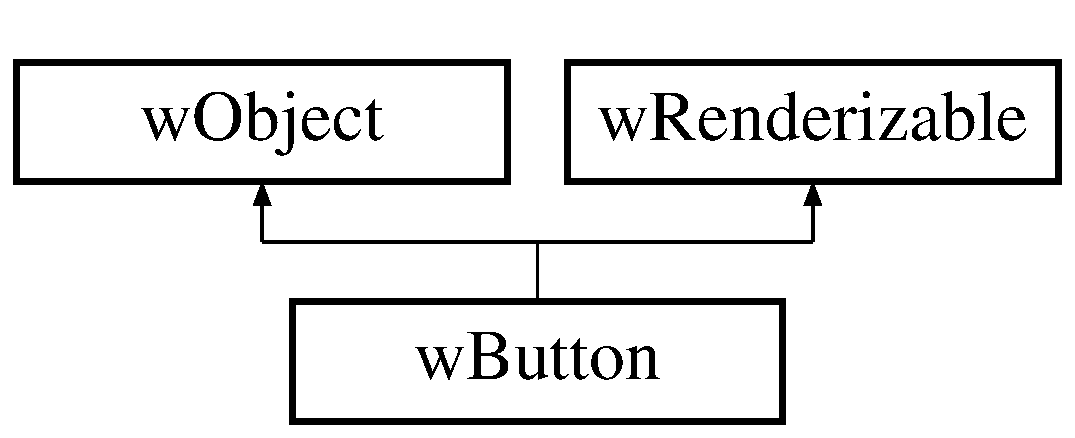
\includegraphics[height=2.000000cm]{classwButton}
\end{center}
\end{figure}
\subsection*{Public Member Functions}
\begin{DoxyCompactItemize}
\item 
\hypertarget{classwButton_ae1900cf64a51d0ccc4e9fe46c0e8ad3c}{
{\bfseries \_\-\_\-construct} (\$name=null, \&\$parent, \$label=\char`\"{}Button\char`\"{})}
\label{classwButton_ae1900cf64a51d0ccc4e9fe46c0e8ad3c}

\item 
\hypertarget{classwButton_afa51efa71e726ced911b25826ba7f164}{
{\bfseries render} ()}
\label{classwButton_afa51efa71e726ced911b25826ba7f164}

\item 
\hypertarget{classwButton_a3badb068eb0f51744c3cb18389ad786d}{
{\bfseries \_\-setDefaults} ()}
\label{classwButton_a3badb068eb0f51744c3cb18389ad786d}

\item 
\hypertarget{classwButton_ac95d2874e371e3c6fc2d4d39cc9e8daf}{
{\bfseries setSelectedValue} (\$data)}
\label{classwButton_ac95d2874e371e3c6fc2d4d39cc9e8daf}

\end{DoxyCompactItemize}
\subsection*{Public Attributes}
\begin{DoxyCompactItemize}
\item 
\hypertarget{classwButton_a847efe4fc21eab72c010dc37c8a3b830}{
{\bfseries \$name} = \char`\"{}\char`\"{}}
\label{classwButton_a847efe4fc21eab72c010dc37c8a3b830}

\item 
\hypertarget{classwButton_a2f775d34d30c98f26d12ecf16c6dab84}{
{\bfseries \$label} = \char`\"{}Button\char`\"{}}
\label{classwButton_a2f775d34d30c98f26d12ecf16c6dab84}

\end{DoxyCompactItemize}


\subsection{Detailed Description}


Definition at line 3 of file wButton.php.



The documentation for this class was generated from the following file:\begin{DoxyCompactItemize}
\item 
wButton.php\end{DoxyCompactItemize}

\hypertarget{classwCheckBox}{
\section{wCheckBox Class Reference}
\label{classwCheckBox}\index{wCheckBox@{wCheckBox}}
}
Inheritance diagram for wCheckBox:\begin{figure}[H]
\begin{center}
\leavevmode
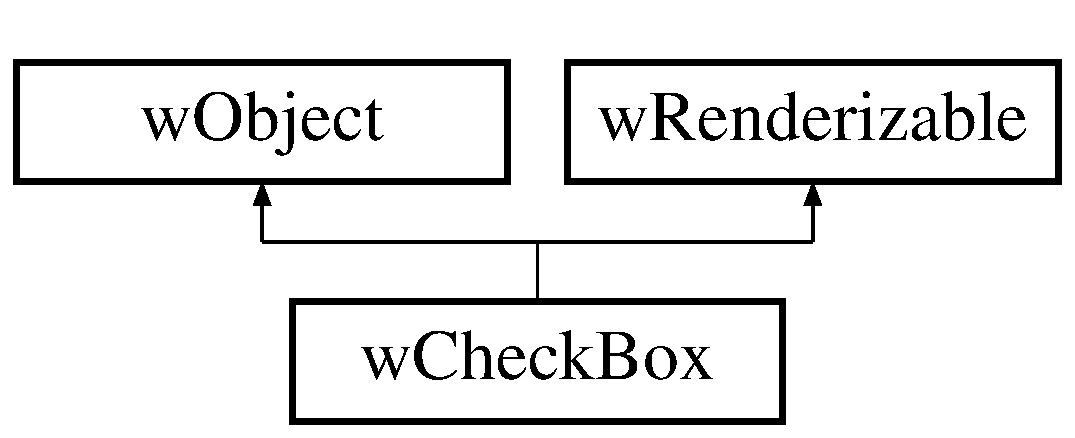
\includegraphics[height=2.000000cm]{classwCheckBox}
\end{center}
\end{figure}
\subsection*{Public Member Functions}
\begin{DoxyCompactItemize}
\item 
\hypertarget{classwCheckBox_abe2e9ab5d730fc2cde13c618ad7ef8dd}{
{\bfseries \_\-\_\-construct} (\$name=null, \&\$parent, \$addPrefix=true)}
\label{classwCheckBox_abe2e9ab5d730fc2cde13c618ad7ef8dd}

\item 
\hypertarget{classwCheckBox_a0fd9ab2d9eee80f87fd17c15fb85ff54}{
{\bfseries render} ()}
\label{classwCheckBox_a0fd9ab2d9eee80f87fd17c15fb85ff54}

\item 
\hypertarget{classwCheckBox_acb4ad73eddd9b47317a96c30b604d469}{
{\bfseries \_\-setDefaults} ()}
\label{classwCheckBox_acb4ad73eddd9b47317a96c30b604d469}

\item 
\hypertarget{classwCheckBox_a903a74c0dfe2b815f5130c2d494b3a0b}{
{\bfseries setDataModel} (\$data)}
\label{classwCheckBox_a903a74c0dfe2b815f5130c2d494b3a0b}

\item 
\hypertarget{classwCheckBox_a4a69292303dfba7a8728019c11e33335}{
{\bfseries setSelectedIndex} (\$i)}
\label{classwCheckBox_a4a69292303dfba7a8728019c11e33335}

\end{DoxyCompactItemize}
\subsection*{Public Attributes}
\begin{DoxyCompactItemize}
\item 
\hypertarget{classwCheckBox_a9c07fe7a31f2502adcb4ae93e80c3f7f}{
{\bfseries \$name} = \char`\"{}\char`\"{}}
\label{classwCheckBox_a9c07fe7a31f2502adcb4ae93e80c3f7f}

\item 
\hypertarget{classwCheckBox_a58137333c3f18572be96d11b2ec5e13e}{
{\bfseries \$value} = \char`\"{}\char`\"{}}
\label{classwCheckBox_a58137333c3f18572be96d11b2ec5e13e}

\end{DoxyCompactItemize}


\subsection{Detailed Description}


Definition at line 3 of file wCheckBox.php.



The documentation for this class was generated from the following file:\begin{DoxyCompactItemize}
\item 
wCheckBox.php\end{DoxyCompactItemize}

\hypertarget{classwFile}{
\section{wFile Class Reference}
\label{classwFile}\index{wFile@{wFile}}
}
Inheritance diagram for wFile:\begin{figure}[H]
\begin{center}
\leavevmode
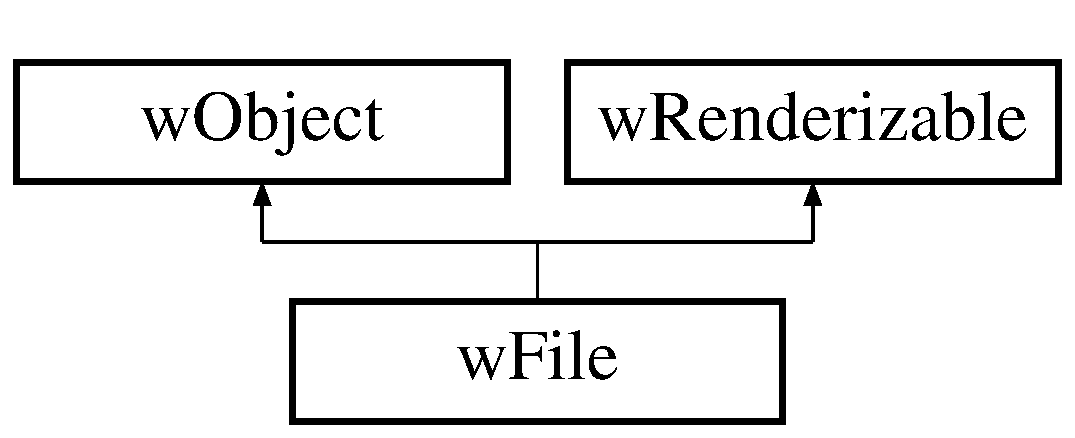
\includegraphics[height=2.000000cm]{classwFile}
\end{center}
\end{figure}
\subsection*{Public Member Functions}
\begin{DoxyCompactItemize}
\item 
\hypertarget{classwFile_ae8cab8f05a7f3edc7f823a9cee93b801}{
{\bfseries \_\-\_\-construct} (\$name=null, \&\$parent)}
\label{classwFile_ae8cab8f05a7f3edc7f823a9cee93b801}

\item 
\hypertarget{classwFile_a9575007036cb44bee5cf726fc1a9441d}{
{\bfseries render} ()}
\label{classwFile_a9575007036cb44bee5cf726fc1a9441d}

\item 
\hypertarget{classwFile_a5a1cec28d059f7d4e700fa6456e14980}{
{\bfseries \_\-setDefaults} ()}
\label{classwFile_a5a1cec28d059f7d4e700fa6456e14980}

\item 
\hypertarget{classwFile_a021668e35de9bef5a80f588b7e6ef944}{
{\bfseries setSelectedValue} (\$data)}
\label{classwFile_a021668e35de9bef5a80f588b7e6ef944}

\end{DoxyCompactItemize}
\subsection*{Public Attributes}
\begin{DoxyCompactItemize}
\item 
\hypertarget{classwFile_afa68dc5e8738a79115f8f8098915ed4e}{
{\bfseries \$name} = \char`\"{}\char`\"{}}
\label{classwFile_afa68dc5e8738a79115f8f8098915ed4e}

\item 
\hypertarget{classwFile_a5d3a7e1abb181c5541813f3027d35608}{
{\bfseries \$value} = \char`\"{}\char`\"{}}
\label{classwFile_a5d3a7e1abb181c5541813f3027d35608}

\item 
\hypertarget{classwFile_a66c4306b6befacf893aba921b04d9db8}{
{\bfseries \$maxlenght} = \char`\"{}\char`\"{}}
\label{classwFile_a66c4306b6befacf893aba921b04d9db8}

\end{DoxyCompactItemize}


\subsection{Detailed Description}


Definition at line 3 of file wFile.php.



The documentation for this class was generated from the following file:\begin{DoxyCompactItemize}
\item 
wFile.php\end{DoxyCompactItemize}

\hypertarget{classwFileShow}{
\section{wFileShow Class Reference}
\label{classwFileShow}\index{wFileShow@{wFileShow}}
}
Inheritance diagram for wFileShow:\begin{figure}[H]
\begin{center}
\leavevmode
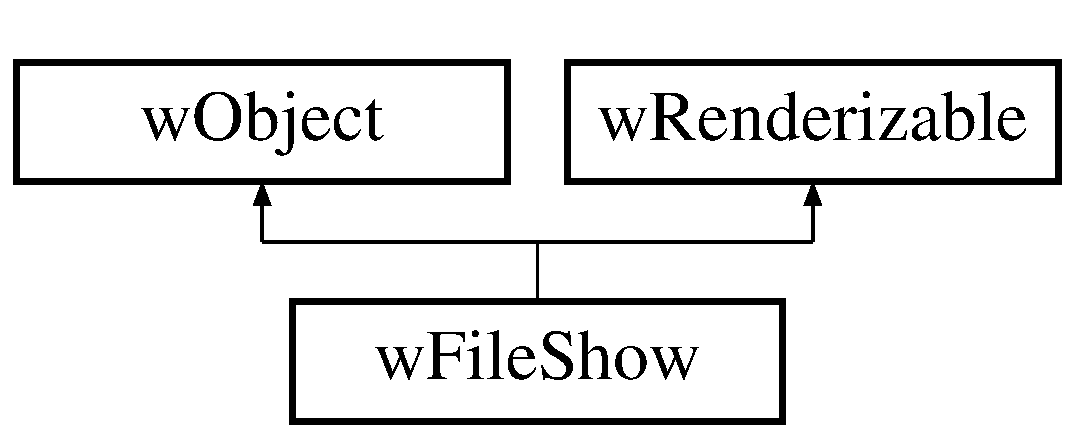
\includegraphics[height=2.000000cm]{classwFileShow}
\end{center}
\end{figure}
\subsection*{Public Member Functions}
\begin{DoxyCompactItemize}
\item 
\hypertarget{classwFileShow_ac9714f8ec7a874634dc1ef287c071ef0}{
{\bfseries \_\-\_\-construct} (\$name=null, \$parent, \$addPrefix=true)}
\label{classwFileShow_ac9714f8ec7a874634dc1ef287c071ef0}

\item 
\hypertarget{classwFileShow_ad22a26cbe218296e36fe1c48c32f05b9}{
{\bfseries render} ()}
\label{classwFileShow_ad22a26cbe218296e36fe1c48c32f05b9}

\item 
\hypertarget{classwFileShow_af4331bffca885f8b30d02013a7d8510a}{
{\bfseries \_\-setDefaults} ()}
\label{classwFileShow_af4331bffca885f8b30d02013a7d8510a}

\item 
\hypertarget{classwFileShow_a9f157babb9bd0c5b88670ed89a3531d6}{
{\bfseries setSelectedValue} (\$data)}
\label{classwFileShow_a9f157babb9bd0c5b88670ed89a3531d6}

\end{DoxyCompactItemize}
\subsection*{Public Attributes}
\begin{DoxyCompactItemize}
\item 
\hypertarget{classwFileShow_a7cb7cb1f8a1a63cc58bfae35b4d3b0e1}{
{\bfseries \$name} = \char`\"{}\char`\"{}}
\label{classwFileShow_a7cb7cb1f8a1a63cc58bfae35b4d3b0e1}

\item 
\hypertarget{classwFileShow_af9bad721eb1965e28425293be077d0c1}{
{\bfseries \$label} = \char`\"{}Button\char`\"{}}
\label{classwFileShow_af9bad721eb1965e28425293be077d0c1}

\item 
\hypertarget{classwFileShow_a2d70e3621919385dd5e342c8b6020ddc}{
{\bfseries \$src} = \char`\"{}\char`\"{}}
\label{classwFileShow_a2d70e3621919385dd5e342c8b6020ddc}

\item 
\hypertarget{classwFileShow_afaa5b90cfa019acbf02badd102295c33}{
{\bfseries \$idfile} = \char`\"{}\char`\"{}}
\label{classwFileShow_afaa5b90cfa019acbf02badd102295c33}

\item 
\hypertarget{classwFileShow_ad1a9655f9046ea108b06781e95d950e0}{
{\bfseries \$id}}
\label{classwFileShow_ad1a9655f9046ea108b06781e95d950e0}

\end{DoxyCompactItemize}


\subsection{Detailed Description}


Definition at line 3 of file wFileShow.php.



The documentation for this class was generated from the following file:\begin{DoxyCompactItemize}
\item 
wFileShow.php\end{DoxyCompactItemize}

\hypertarget{classwFileUpload}{
\section{wFileUpload Class Reference}
\label{classwFileUpload}\index{wFileUpload@{wFileUpload}}
}
Inheritance diagram for wFileUpload:\begin{figure}[H]
\begin{center}
\leavevmode
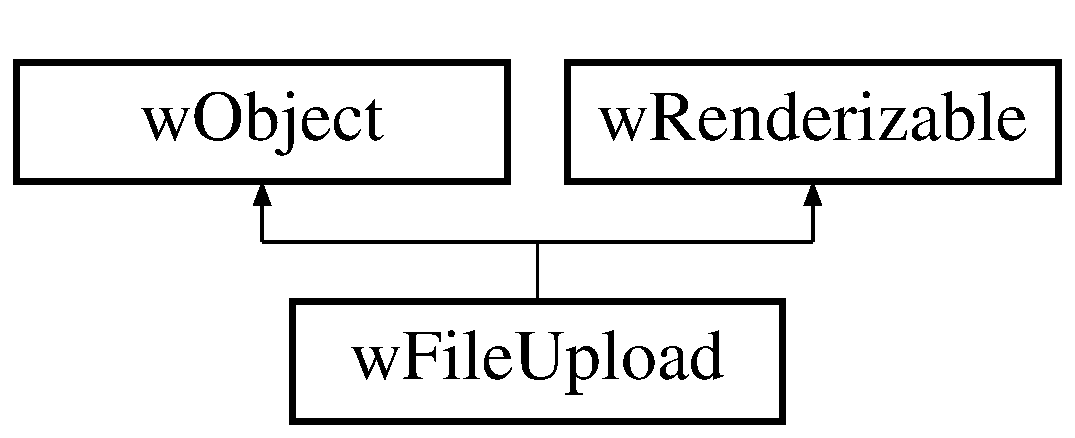
\includegraphics[height=2.000000cm]{classwFileUpload}
\end{center}
\end{figure}
\subsection*{Public Member Functions}
\begin{DoxyCompactItemize}
\item 
\hypertarget{classwFileUpload_a0b9a0b67426fead321433a82bebca839}{
{\bfseries \_\-\_\-construct} (\$name=null, \&\$parent)}
\label{classwFileUpload_a0b9a0b67426fead321433a82bebca839}

\item 
\hypertarget{classwFileUpload_a823542516049056a7c6b3d41d5692362}{
{\bfseries render} ()}
\label{classwFileUpload_a823542516049056a7c6b3d41d5692362}

\item 
\hypertarget{classwFileUpload_a0bba5d5dda74c9c2c337a50efab36bc7}{
{\bfseries \_\-setDefaults} ()}
\label{classwFileUpload_a0bba5d5dda74c9c2c337a50efab36bc7}

\item 
\hypertarget{classwFileUpload_a67492ce12aebdbaf10c04326640dcce3}{
{\bfseries setSelectedValue} (\$data)}
\label{classwFileUpload_a67492ce12aebdbaf10c04326640dcce3}

\end{DoxyCompactItemize}
\subsection*{Public Attributes}
\begin{DoxyCompactItemize}
\item 
\hypertarget{classwFileUpload_a5d338205c03c0f0eae5904a34a6307c9}{
{\bfseries \$name} = \char`\"{}\char`\"{}}
\label{classwFileUpload_a5d338205c03c0f0eae5904a34a6307c9}

\item 
\hypertarget{classwFileUpload_a961f77760208dc6194b31ae721017a95}{
{\bfseries \$value} = \char`\"{}\char`\"{}}
\label{classwFileUpload_a961f77760208dc6194b31ae721017a95}

\item 
\hypertarget{classwFileUpload_ad6ac17f433f473fa4f0c800830ded303}{
{\bfseries \$maxlenght} = \char`\"{}\char`\"{}}
\label{classwFileUpload_ad6ac17f433f473fa4f0c800830ded303}

\item 
\hypertarget{classwFileUpload_a6983bb9cf787dc6beb62faba6661ad48}{
{\bfseries \$tipo} = \char`\"{}\char`\"{}}
\label{classwFileUpload_a6983bb9cf787dc6beb62faba6661ad48}

\end{DoxyCompactItemize}


\subsection{Detailed Description}


Definition at line 3 of file wFileUpload.php.



The documentation for this class was generated from the following file:\begin{DoxyCompactItemize}
\item 
wFileUpload.php\end{DoxyCompactItemize}

\hypertarget{classwFileUploadtwo}{
\section{wFileUploadtwo Class Reference}
\label{classwFileUploadtwo}\index{wFileUploadtwo@{wFileUploadtwo}}
}
Inheritance diagram for wFileUploadtwo:\begin{figure}[H]
\begin{center}
\leavevmode
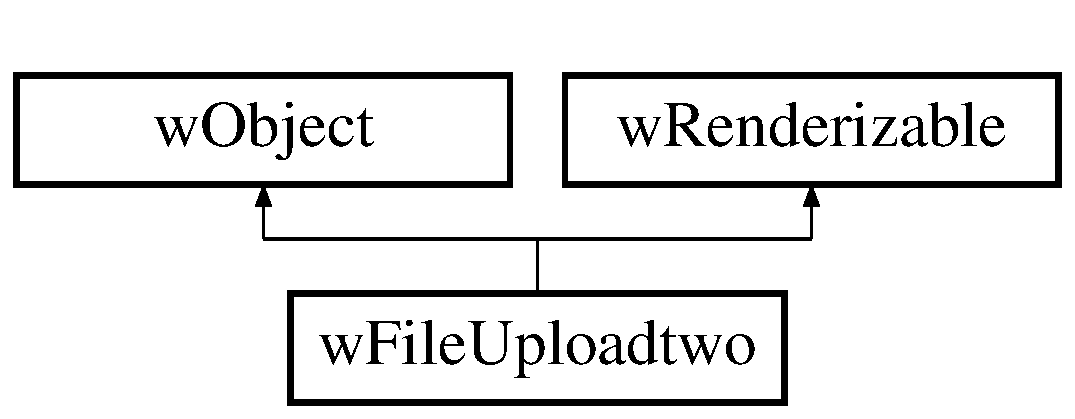
\includegraphics[height=2.000000cm]{classwFileUploadtwo}
\end{center}
\end{figure}
\subsection*{Public Member Functions}
\begin{DoxyCompactItemize}
\item 
\hypertarget{classwFileUploadtwo_a3113c74facfa0d105d0c8269216db92c}{
{\bfseries \_\-\_\-construct} (\$name=null, \&\$parent)}
\label{classwFileUploadtwo_a3113c74facfa0d105d0c8269216db92c}

\item 
\hypertarget{classwFileUploadtwo_a6b6a5f8b9c423966b90832a511ef173d}{
{\bfseries render} ()}
\label{classwFileUploadtwo_a6b6a5f8b9c423966b90832a511ef173d}

\item 
\hypertarget{classwFileUploadtwo_aeaf4ef4719c9695bd0ec5488f874c2da}{
{\bfseries \_\-setDefaults} ()}
\label{classwFileUploadtwo_aeaf4ef4719c9695bd0ec5488f874c2da}

\item 
\hypertarget{classwFileUploadtwo_a8d947b19aa8cd48839bfdb313f22a996}{
{\bfseries setSelectedValue} (\$data)}
\label{classwFileUploadtwo_a8d947b19aa8cd48839bfdb313f22a996}

\end{DoxyCompactItemize}
\subsection*{Public Attributes}
\begin{DoxyCompactItemize}
\item 
\hypertarget{classwFileUploadtwo_ac34c4b8e1796a1df09b6b3e56770c437}{
{\bfseries \$name} = \char`\"{}\char`\"{}}
\label{classwFileUploadtwo_ac34c4b8e1796a1df09b6b3e56770c437}

\item 
\hypertarget{classwFileUploadtwo_a8f3b45b500557f5bf717a8ed4b35809c}{
{\bfseries \$value} = \char`\"{}\char`\"{}}
\label{classwFileUploadtwo_a8f3b45b500557f5bf717a8ed4b35809c}

\item 
\hypertarget{classwFileUploadtwo_a77d70a4521eaa8df2f6a648047a1cf44}{
{\bfseries \$maxlenght} = \char`\"{}\char`\"{}}
\label{classwFileUploadtwo_a77d70a4521eaa8df2f6a648047a1cf44}

\end{DoxyCompactItemize}


\subsection{Detailed Description}


Definition at line 3 of file wFileUploadtwo.php.



The documentation for this class was generated from the following file:\begin{DoxyCompactItemize}
\item 
wFileUploadtwo.php\end{DoxyCompactItemize}

\hypertarget{classwForm}{
\section{wForm Class Reference}
\label{classwForm}\index{wForm@{wForm}}
}
Inheritance diagram for wForm:\begin{figure}[H]
\begin{center}
\leavevmode
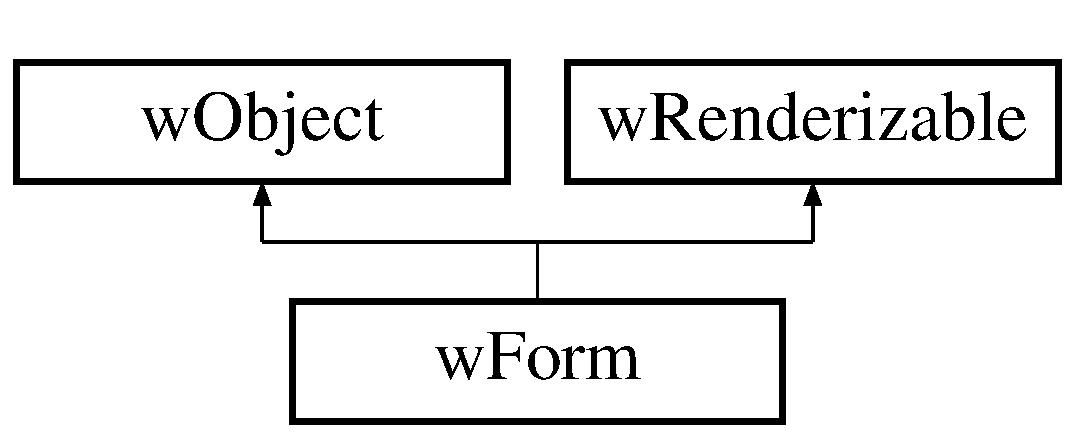
\includegraphics[height=2.000000cm]{classwForm}
\end{center}
\end{figure}
\subsection*{Public Member Functions}
\begin{DoxyCompactItemize}
\item 
\hypertarget{classwForm_aaaa7f4f4ddacfce6d6d085bd905d7aa4}{
{\bfseries \_\-\_\-construct} (\$name=null, \&\$parent)}
\label{classwForm_aaaa7f4f4ddacfce6d6d085bd905d7aa4}

\item 
\hypertarget{classwForm_a138cc0db418e51d3f4d1c750f5b17cd1}{
{\bfseries createDefaultButtons} ()}
\label{classwForm_a138cc0db418e51d3f4d1c750f5b17cd1}

\item 
\hypertarget{classwForm_a6e17b60d76e746a73bbd78ef285223ff}{
{\bfseries render} ()}
\label{classwForm_a6e17b60d76e746a73bbd78ef285223ff}

\item 
\hypertarget{classwForm_a8176f0c924f780deef3d61efb13dfb44}{
{\bfseries setDataModelFromCore} (\$object)}
\label{classwForm_a8176f0c924f780deef3d61efb13dfb44}

\item 
\hypertarget{classwForm_a9df1501b0be86c02cb3e3e3bee1c2636}{
{\bfseries \_\-setDefaults} ()}
\label{classwForm_a9df1501b0be86c02cb3e3e3bee1c2636}

\item 
\hypertarget{classwForm_a6e5785cda311a90bc8de041eeeda70a3}{
{\bfseries requestloadFromId} (\$id, \$fjid, \$class)}
\label{classwForm_a6e5785cda311a90bc8de041eeeda70a3}

\item 
\hypertarget{classwForm_a3f211d36d8d044c075f8a5a833504c0b}{
{\bfseries requestSaveForm} (\$id, \$fjid, \$data)}
\label{classwForm_a3f211d36d8d044c075f8a5a833504c0b}

\item 
\hypertarget{classwForm_a5b51cb0d43f95baa6b681daa21df1bba}{
{\bfseries requestDeleteForm} (\$id, \$fjid, \$data)}
\label{classwForm_a5b51cb0d43f95baa6b681daa21df1bba}

\item 
\hypertarget{classwForm_a8d56069f01d853007f060d94edb4968e}{
{\bfseries requestNewForm} (\$id, \$fjid)}
\label{classwForm_a8d56069f01d853007f060d94edb4968e}

\item 
\hypertarget{classwForm_a7270b4f28aa9961f880b8a70e6fbcc67}{
{\bfseries doAfterSave} (\$method)}
\label{classwForm_a7270b4f28aa9961f880b8a70e6fbcc67}

\item 
\hypertarget{classwForm_ad028831ef99607be062ee095b0ac18f3}{
{\bfseries doAfterDelete} (\$method)}
\label{classwForm_ad028831ef99607be062ee095b0ac18f3}

\end{DoxyCompactItemize}
\subsection*{Static Public Member Functions}
\begin{DoxyCompactItemize}
\item 
\hypertarget{classwForm_a159417635f66929192885f5f71cb2346}{
static {\bfseries dataFormater} (\$value, \$type)}
\label{classwForm_a159417635f66929192885f5f71cb2346}

\end{DoxyCompactItemize}
\subsection*{Public Attributes}
\begin{DoxyCompactItemize}
\item 
\hypertarget{classwForm_a3a25cf4996fc31fa9f55e8792548c431}{
{\bfseries \$name} = \char`\"{}\char`\"{}}
\label{classwForm_a3a25cf4996fc31fa9f55e8792548c431}

\item 
\hypertarget{classwForm_a3d5269aef844a7df3e3f3bc792b01204}{
{\bfseries \$coreObject} = null}
\label{classwForm_a3d5269aef844a7df3e3f3bc792b01204}

\item 
\hypertarget{classwForm_a9b30b0eded4585b27c7caceee6bce188}{
{\bfseries \$afterSaveMethod} = null}
\label{classwForm_a9b30b0eded4585b27c7caceee6bce188}

\end{DoxyCompactItemize}


\subsection{Detailed Description}


Definition at line 3 of file wForm.php.



The documentation for this class was generated from the following file:\begin{DoxyCompactItemize}
\item 
wForm.php\end{DoxyCompactItemize}

\hypertarget{classwGrid}{
\section{wGrid Class Reference}
\label{classwGrid}\index{wGrid@{wGrid}}
}
Inheritance diagram for wGrid:\begin{figure}[H]
\begin{center}
\leavevmode
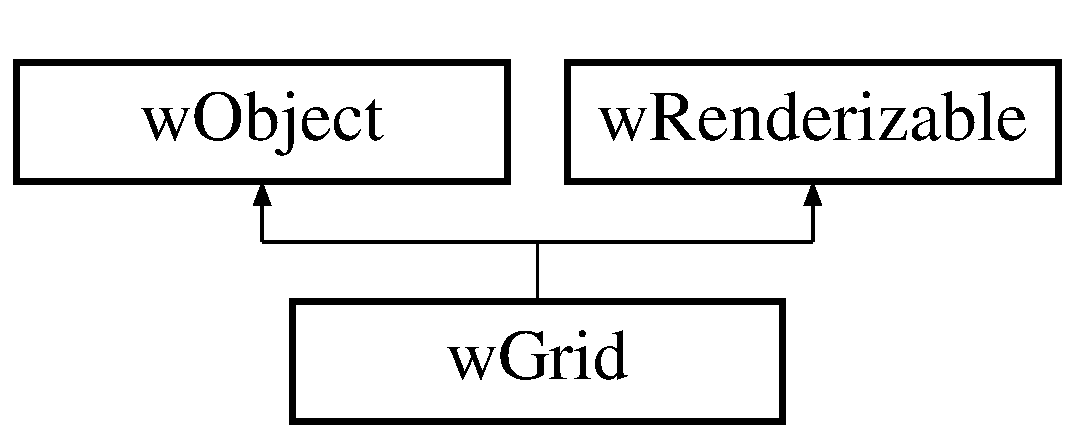
\includegraphics[height=2.000000cm]{classwGrid}
\end{center}
\end{figure}
\subsection*{Public Member Functions}
\begin{DoxyCompactItemize}
\item 
\hypertarget{classwGrid_a1d89d52f6fdeef2554b048e60c4d8dce}{
{\bfseries \_\-\_\-construct} (\$name=null, \&\$parent)}
\label{classwGrid_a1d89d52f6fdeef2554b048e60c4d8dce}

\item 
\hypertarget{classwGrid_a28b78e7e9e0b04ca04567e6730cc3b7a}{
{\bfseries addColumn} (\$col)}
\label{classwGrid_a28b78e7e9e0b04ca04567e6730cc3b7a}

\item 
\hypertarget{classwGrid_a258b2db6ee09caefbbc1b4d0003225c1}{
{\bfseries render} ()}
\label{classwGrid_a258b2db6ee09caefbbc1b4d0003225c1}

\item 
\hypertarget{classwGrid_a6a5f92dceb5d88489946f65899c2c0fa}{
{\bfseries setWidth} (\$w)}
\label{classwGrid_a6a5f92dceb5d88489946f65899c2c0fa}

\item 
\hypertarget{classwGrid_aac676085e3b4ccb59e7ce4f12520407a}{
{\bfseries \_\-setDefaults} ()}
\label{classwGrid_aac676085e3b4ccb59e7ce4f12520407a}

\item 
\hypertarget{classwGrid_a6eb2fb6789b3779a0f7621b3543a84b9}{
{\bfseries setDataModel} (\$model)}
\label{classwGrid_a6eb2fb6789b3779a0f7621b3543a84b9}

\item 
\hypertarget{classwGrid_a994a94498abda48a1a05b1f8b33b5cf5}{
{\bfseries setDataModelFromCore} (\$object)}
\label{classwGrid_a994a94498abda48a1a05b1f8b33b5cf5}

\end{DoxyCompactItemize}
\subsection*{Static Public Member Functions}
\begin{DoxyCompactItemize}
\item 
\hypertarget{classwGrid_a28f16946248bc8fdc240234f4d9531e0}{
static {\bfseries prepareGridData} (\$resultados, \$nRes, \$pagina=1)}
\label{classwGrid_a28f16946248bc8fdc240234f4d9531e0}

\end{DoxyCompactItemize}
\subsection*{Public Attributes}
\begin{DoxyCompactItemize}
\item 
\hypertarget{classwGrid_aec5c20eab9f71c8cbd2c7010061dd6f2}{
{\bfseries \$name} = \char`\"{}\char`\"{}}
\label{classwGrid_aec5c20eab9f71c8cbd2c7010061dd6f2}

\item 
\hypertarget{classwGrid_a0a49e2985d586e7ec5d31b3d5a71c8fd}{
{\bfseries \$type} = 0}
\label{classwGrid_a0a49e2985d586e7ec5d31b3d5a71c8fd}

\item 
\hypertarget{classwGrid_ab86f1ebf27b016652b711ffb97079dea}{
{\bfseries \$dataModel} = array()}
\label{classwGrid_ab86f1ebf27b016652b711ffb97079dea}

\item 
\hypertarget{classwGrid_ae44802db87dacddace57515a28d47cda}{
{\bfseries \$DataURL}}
\label{classwGrid_ae44802db87dacddace57515a28d47cda}

\item 
\hypertarget{classwGrid_a0457cd26d2357e132a3fd7cebf679967}{
{\bfseries \$columns}}
\label{classwGrid_a0457cd26d2357e132a3fd7cebf679967}

\item 
\hypertarget{classwGrid_ab9e7d668bf54e132059a93d12965bc62}{
{\bfseries \$title}}
\label{classwGrid_ab9e7d668bf54e132059a93d12965bc62}

\item 
\hypertarget{classwGrid_a8322680e99fd7e35572b49720ed849da}{
{\bfseries \$width}}
\label{classwGrid_a8322680e99fd7e35572b49720ed849da}

\item 
\hypertarget{classwGrid_a78c1d8b21816659cb25f274b5fcfa88e}{
{\bfseries \$actionOnSelectID} = \char`\"{}a=1\char`\"{}}
\label{classwGrid_a78c1d8b21816659cb25f274b5fcfa88e}

\end{DoxyCompactItemize}


\subsection{Detailed Description}


Definition at line 3 of file wGrid.php.



The documentation for this class was generated from the following file:\begin{DoxyCompactItemize}
\item 
wGrid.php\end{DoxyCompactItemize}

\hypertarget{classwHidden}{
\section{wHidden Class Reference}
\label{classwHidden}\index{wHidden@{wHidden}}
}
Inheritance diagram for wHidden:\begin{figure}[H]
\begin{center}
\leavevmode
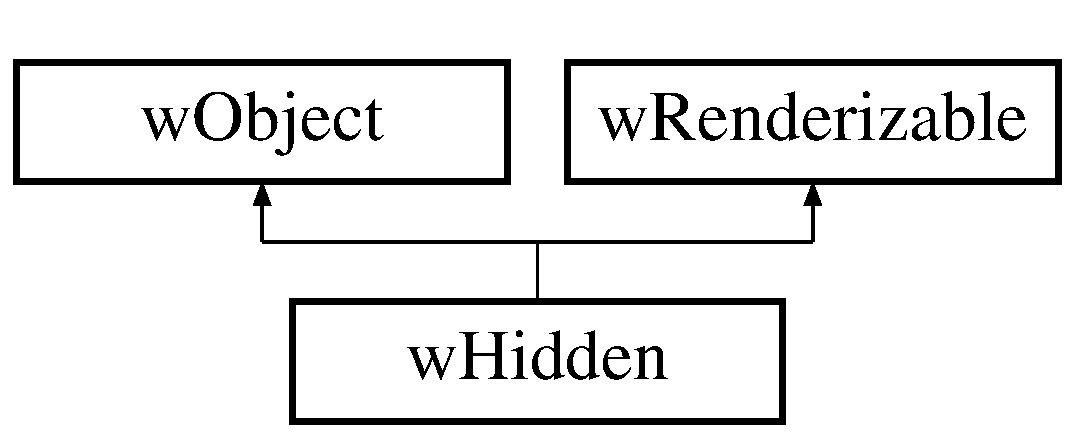
\includegraphics[height=2.000000cm]{classwHidden}
\end{center}
\end{figure}
\subsection*{Public Member Functions}
\begin{DoxyCompactItemize}
\item 
\hypertarget{classwHidden_af52f2782a69582ed2b435e25d81867ca}{
{\bfseries \_\-\_\-construct} (\$name=null, \&\$parent, \$addPrefix=true)}
\label{classwHidden_af52f2782a69582ed2b435e25d81867ca}

\item 
\hypertarget{classwHidden_a61f2b2f60a9e2f72e79bec91b59bf135}{
{\bfseries render} ()}
\label{classwHidden_a61f2b2f60a9e2f72e79bec91b59bf135}

\item 
\hypertarget{classwHidden_acc6abbf19048aeae0a17d7db83a370e4}{
{\bfseries setSelectedValue} (\$data)}
\label{classwHidden_acc6abbf19048aeae0a17d7db83a370e4}

\end{DoxyCompactItemize}
\subsection*{Public Attributes}
\begin{DoxyCompactItemize}
\item 
\hypertarget{classwHidden_a3c7d143be7addb0f0b33c904a634788c}{
{\bfseries \$name} = \char`\"{}\char`\"{}}
\label{classwHidden_a3c7d143be7addb0f0b33c904a634788c}

\item 
\hypertarget{classwHidden_a61338ec10362c659edbe1e0cabf055b9}{
{\bfseries \$value} = \char`\"{}\char`\"{}}
\label{classwHidden_a61338ec10362c659edbe1e0cabf055b9}

\item 
\hypertarget{classwHidden_ad781727984fe8efd282debcb4ee190a2}{
{\bfseries \$maxlenght} = \char`\"{}\char`\"{}}
\label{classwHidden_ad781727984fe8efd282debcb4ee190a2}

\end{DoxyCompactItemize}


\subsection{Detailed Description}


Definition at line 3 of file wHidden.php.



The documentation for this class was generated from the following file:\begin{DoxyCompactItemize}
\item 
wHidden.php\end{DoxyCompactItemize}

\hypertarget{classwHTML}{
\section{wHTML Class Reference}
\label{classwHTML}\index{wHTML@{wHTML}}
}
Inheritance diagram for wHTML:\begin{figure}[H]
\begin{center}
\leavevmode
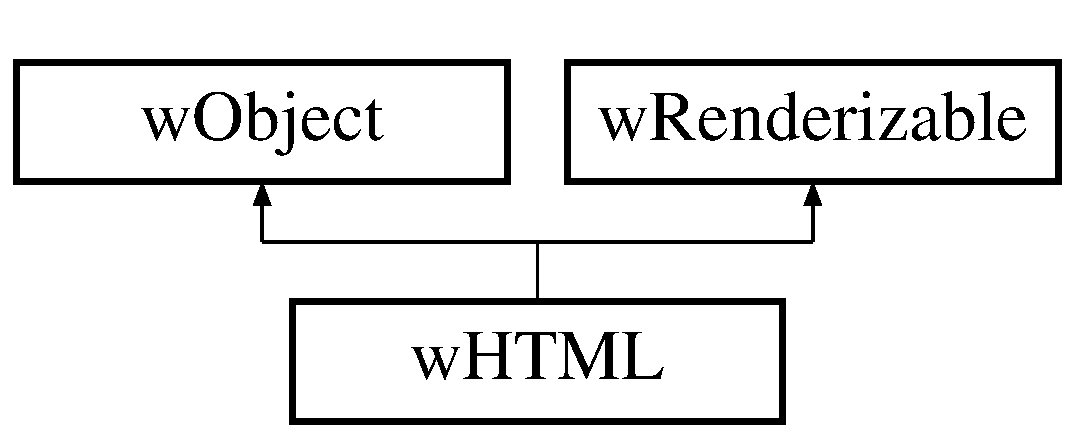
\includegraphics[height=2.000000cm]{classwHTML}
\end{center}
\end{figure}
\subsection*{Public Member Functions}
\begin{DoxyCompactItemize}
\item 
\hypertarget{classwHTML_a75691dde71b4ccdfb73765e5d844e3d3}{
{\bfseries setHTML} (\$HTML)}
\label{classwHTML_a75691dde71b4ccdfb73765e5d844e3d3}

\item 
\hypertarget{classwHTML_a1431f340790d3b3e223ea43849877fd2}{
{\bfseries render} ()}
\label{classwHTML_a1431f340790d3b3e223ea43849877fd2}

\item 
\hypertarget{classwHTML_a10bcae073ee26ce8481c4f990881b1cb}{
{\bfseries \_\-setDefaults} ()}
\label{classwHTML_a10bcae073ee26ce8481c4f990881b1cb}

\end{DoxyCompactItemize}
\subsection*{Public Attributes}
\begin{DoxyCompactItemize}
\item 
\hypertarget{classwHTML_a9b0d0bbdeaa085f9d1daffc942e44fd6}{
{\bfseries \$content}}
\label{classwHTML_a9b0d0bbdeaa085f9d1daffc942e44fd6}

\item 
\hypertarget{classwHTML_a8391ae7c486824428775dfcf9c223c7b}{
{\bfseries \$name} = \char`\"{}\char`\"{}}
\label{classwHTML_a8391ae7c486824428775dfcf9c223c7b}

\end{DoxyCompactItemize}


\subsection{Detailed Description}


Definition at line 3 of file wHTML.php.



The documentation for this class was generated from the following file:\begin{DoxyCompactItemize}
\item 
wHTML.php\end{DoxyCompactItemize}

\hypertarget{classwImage}{
\section{wImage Class Reference}
\label{classwImage}\index{wImage@{wImage}}
}
Inheritance diagram for wImage:\begin{figure}[H]
\begin{center}
\leavevmode
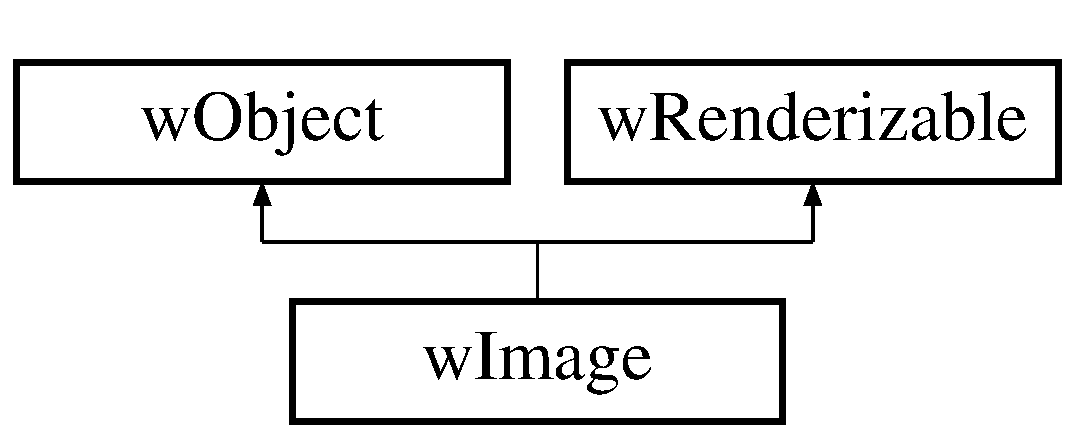
\includegraphics[height=2.000000cm]{classwImage}
\end{center}
\end{figure}
\subsection*{Public Member Functions}
\begin{DoxyCompactItemize}
\item 
\hypertarget{classwImage_ad04ab34237d290d5270d432e5c74d60c}{
{\bfseries \_\-\_\-construct} (\$name=null, \$parent, \$addPrefix=true)}
\label{classwImage_ad04ab34237d290d5270d432e5c74d60c}

\item 
\hypertarget{classwImage_a9a7c7b21b64fc355af8b9a09545813a1}{
{\bfseries render} ()}
\label{classwImage_a9a7c7b21b64fc355af8b9a09545813a1}

\item 
\hypertarget{classwImage_a0a9240d24e243ad9e679d05c3a426b70}{
{\bfseries \_\-setDefaults} ()}
\label{classwImage_a0a9240d24e243ad9e679d05c3a426b70}

\item 
\hypertarget{classwImage_adbcf8345c605d938ecbe34b893943987}{
{\bfseries setSelectedValue} (\$data)}
\label{classwImage_adbcf8345c605d938ecbe34b893943987}

\end{DoxyCompactItemize}
\subsection*{Public Attributes}
\begin{DoxyCompactItemize}
\item 
\hypertarget{classwImage_a8f91fdb684d8f5af4bcf1a1835eb079e}{
{\bfseries \$name} = \char`\"{}\char`\"{}}
\label{classwImage_a8f91fdb684d8f5af4bcf1a1835eb079e}

\item 
\hypertarget{classwImage_a949954048364902dba73ec70ae6f2c32}{
{\bfseries \$label} = \char`\"{}Button\char`\"{}}
\label{classwImage_a949954048364902dba73ec70ae6f2c32}

\item 
\hypertarget{classwImage_a41c2848c583c9d707a70be54b0e97e0f}{
{\bfseries \$src} = \char`\"{}\char`\"{}}
\label{classwImage_a41c2848c583c9d707a70be54b0e97e0f}

\item 
\hypertarget{classwImage_ab0ada74249521ae3b02ae6951f44c92e}{
{\bfseries \$click} = \char`\"{}\char`\"{}}
\label{classwImage_ab0ada74249521ae3b02ae6951f44c92e}

\item 
\hypertarget{classwImage_a2cd8bf3c77283f74edb8def5266822b2}{
{\bfseries \$id}}
\label{classwImage_a2cd8bf3c77283f74edb8def5266822b2}

\end{DoxyCompactItemize}


\subsection{Detailed Description}


Definition at line 3 of file wImage.php.



The documentation for this class was generated from the following file:\begin{DoxyCompactItemize}
\item 
wImage.php\end{DoxyCompactItemize}

\hypertarget{classwImageShow}{
\section{wImageShow Class Reference}
\label{classwImageShow}\index{wImageShow@{wImageShow}}
}
Inheritance diagram for wImageShow:\begin{figure}[H]
\begin{center}
\leavevmode
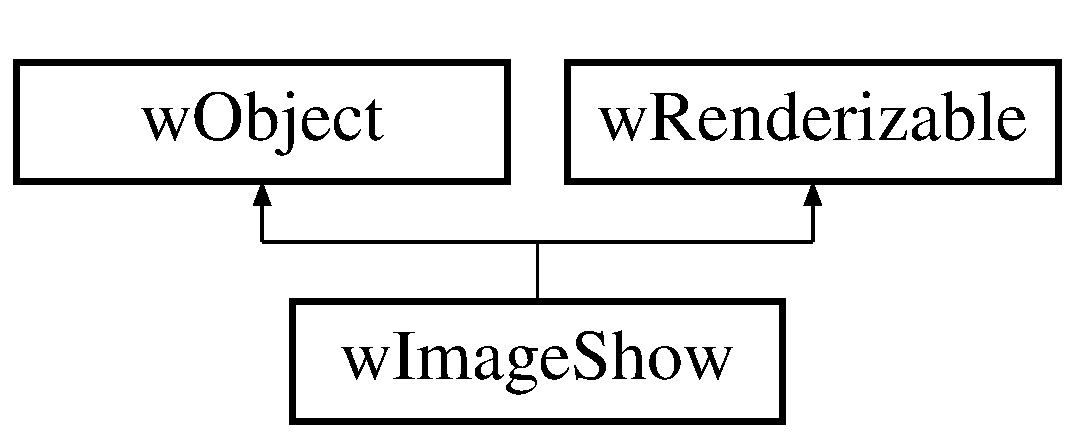
\includegraphics[height=2.000000cm]{classwImageShow}
\end{center}
\end{figure}
\subsection*{Public Member Functions}
\begin{DoxyCompactItemize}
\item 
\hypertarget{classwImageShow_a286a317daf9c583427e763994b1e8aae}{
{\bfseries \_\-\_\-construct} (\$name=null, \$parent, \$addPrefix=true)}
\label{classwImageShow_a286a317daf9c583427e763994b1e8aae}

\item 
\hypertarget{classwImageShow_a6004d59ba067051327e88e40a2c07599}{
{\bfseries render} ()}
\label{classwImageShow_a6004d59ba067051327e88e40a2c07599}

\item 
\hypertarget{classwImageShow_a0c5166f9513959056a2d993750207616}{
{\bfseries \_\-setDefaults} ()}
\label{classwImageShow_a0c5166f9513959056a2d993750207616}

\item 
\hypertarget{classwImageShow_a1f7e3d0cd9e670c817bdf9126ba1e7be}{
{\bfseries setSelectedValue} (\$data)}
\label{classwImageShow_a1f7e3d0cd9e670c817bdf9126ba1e7be}

\end{DoxyCompactItemize}
\subsection*{Public Attributes}
\begin{DoxyCompactItemize}
\item 
\hypertarget{classwImageShow_afb4d0cf98aba576ac56f50e0517730ed}{
{\bfseries \$name} = \char`\"{}\char`\"{}}
\label{classwImageShow_afb4d0cf98aba576ac56f50e0517730ed}

\item 
\hypertarget{classwImageShow_af93d61359f89781ebc46ad91a516a936}{
{\bfseries \$label} = \char`\"{}Button\char`\"{}}
\label{classwImageShow_af93d61359f89781ebc46ad91a516a936}

\item 
\hypertarget{classwImageShow_a6045057ad9637a261ea3d99678808ad1}{
{\bfseries \$src} = \char`\"{}\char`\"{}}
\label{classwImageShow_a6045057ad9637a261ea3d99678808ad1}

\item 
\hypertarget{classwImageShow_a006bf986d545395e0d5c2ab9fd1f827a}{
{\bfseries \$idimage} = \char`\"{}\char`\"{}}
\label{classwImageShow_a006bf986d545395e0d5c2ab9fd1f827a}

\item 
\hypertarget{classwImageShow_a627ce93343a7921a52ff2deef3134a26}{
{\bfseries \$id}}
\label{classwImageShow_a627ce93343a7921a52ff2deef3134a26}

\end{DoxyCompactItemize}


\subsection{Detailed Description}


Definition at line 3 of file wImageShow.php.



The documentation for this class was generated from the following file:\begin{DoxyCompactItemize}
\item 
wImageShow.php\end{DoxyCompactItemize}

\hypertarget{classwInput}{
\section{wInput Class Reference}
\label{classwInput}\index{wInput@{wInput}}
}
Inheritance diagram for wInput:\begin{figure}[H]
\begin{center}
\leavevmode
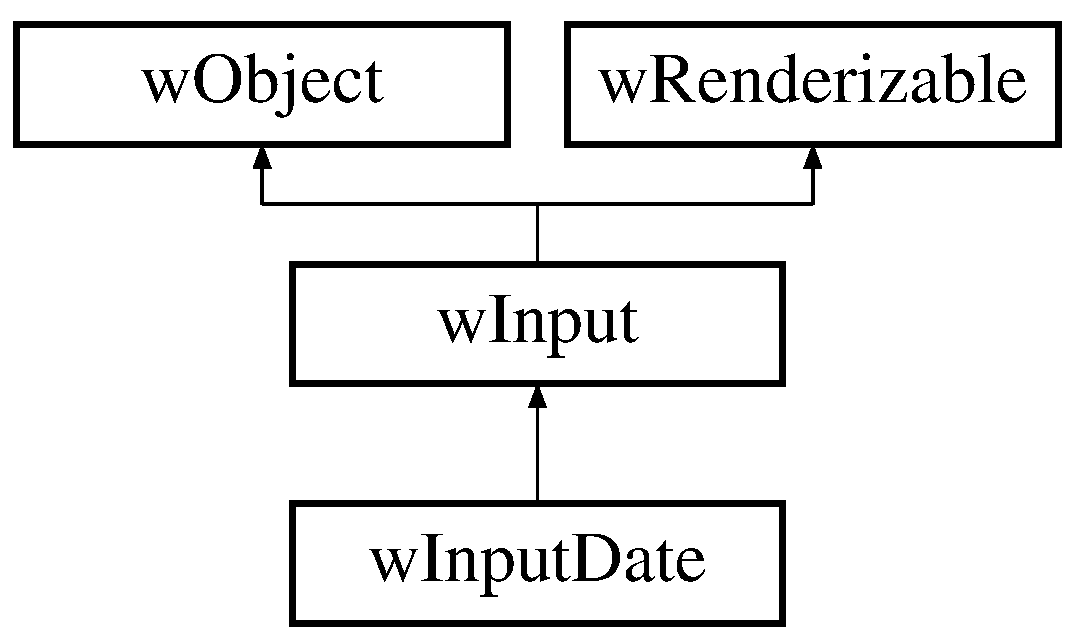
\includegraphics[height=3.000000cm]{classwInput}
\end{center}
\end{figure}
\subsection*{Public Member Functions}
\begin{DoxyCompactItemize}
\item 
\hypertarget{classwInput_a41a19c5dc7c455cbb10cf4ff2bf3472d}{
{\bfseries \_\-\_\-construct} (\$name=null, \&\$parent, \$addPrefix=true)}
\label{classwInput_a41a19c5dc7c455cbb10cf4ff2bf3472d}

\item 
\hypertarget{classwInput_a78266b67a1bcac37ba3163ceed00bd30}{
{\bfseries render} ()}
\label{classwInput_a78266b67a1bcac37ba3163ceed00bd30}

\item 
\hypertarget{classwInput_adb8748e4bc9ad4d403f96c82c0db7f3e}{
{\bfseries \_\-setDefaults} ()}
\label{classwInput_adb8748e4bc9ad4d403f96c82c0db7f3e}

\item 
\hypertarget{classwInput_addbd5fd61e8330493ab9b9a1e652e59c}{
{\bfseries setSelectedValue} (\$data)}
\label{classwInput_addbd5fd61e8330493ab9b9a1e652e59c}

\end{DoxyCompactItemize}
\subsection*{Public Attributes}
\begin{DoxyCompactItemize}
\item 
\hypertarget{classwInput_aad699a854d8db38391bca9cf7b518ff2}{
{\bfseries \$name} = \char`\"{}\char`\"{}}
\label{classwInput_aad699a854d8db38391bca9cf7b518ff2}

\item 
\hypertarget{classwInput_a3c1546fbbafc770d3666ab9f530d9c7f}{
{\bfseries \$value} = \char`\"{}\char`\"{}}
\label{classwInput_a3c1546fbbafc770d3666ab9f530d9c7f}

\item 
\hypertarget{classwInput_ada1d043aad21f34c8729f4904c4a6b76}{
{\bfseries \$maxlenght} = \char`\"{}\char`\"{}}
\label{classwInput_ada1d043aad21f34c8729f4904c4a6b76}

\end{DoxyCompactItemize}


\subsection{Detailed Description}


Definition at line 3 of file wInput.php.



The documentation for this class was generated from the following file:\begin{DoxyCompactItemize}
\item 
wInput.php\end{DoxyCompactItemize}

\hypertarget{classwInputDate}{
\section{wInputDate Class Reference}
\label{classwInputDate}\index{wInputDate@{wInputDate}}
}
Inheritance diagram for wInputDate:\begin{figure}[H]
\begin{center}
\leavevmode
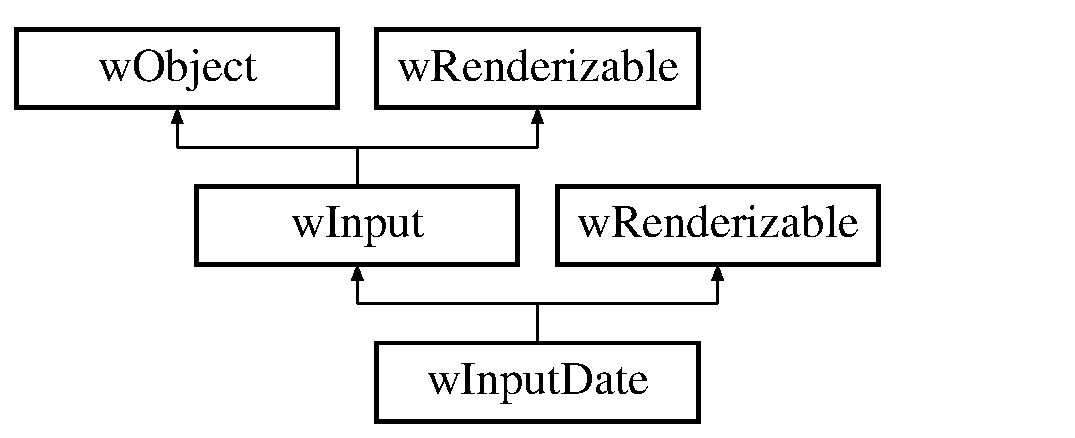
\includegraphics[height=3.000000cm]{classwInputDate}
\end{center}
\end{figure}
\subsection*{Public Member Functions}
\begin{DoxyCompactItemize}
\item 
\hypertarget{classwInputDate_a24005325e5e730cdc3dff26afca8b051}{
{\bfseries \_\-\_\-construct} (\$name=null, \&\$parent, \$addPrefix=true)}
\label{classwInputDate_a24005325e5e730cdc3dff26afca8b051}

\item 
\hypertarget{classwInputDate_ad4a450095e7a28b7cd4c69d693f48dd2}{
{\bfseries render} ()}
\label{classwInputDate_ad4a450095e7a28b7cd4c69d693f48dd2}

\item 
\hypertarget{classwInputDate_a8922d1e6d2cde24dc4dc05794ea1859b}{
{\bfseries \_\-setDefaults} ()}
\label{classwInputDate_a8922d1e6d2cde24dc4dc05794ea1859b}

\item 
\hypertarget{classwInputDate_a9f4597068fdf24ceb8066650cd523714}{
{\bfseries setSelectedValue} (\$data)}
\label{classwInputDate_a9f4597068fdf24ceb8066650cd523714}

\item 
\hypertarget{classwInputDate_a8043b0faea2c624b24ed70cd3d5284b7}{
{\bfseries setTime} (\$time)}
\label{classwInputDate_a8043b0faea2c624b24ed70cd3d5284b7}

\item 
\hypertarget{classwInputDate_af575a0b962a5bd51b95fc9b1369c5daf}{
{\bfseries setFormat} (\$format)}
\label{classwInputDate_af575a0b962a5bd51b95fc9b1369c5daf}

\item 
\hypertarget{classwInputDate_ad346e9139577282de0340f7d249c2fc6}{
{\bfseries ValidateDate} (\$id, \$event, \$myDate)}
\label{classwInputDate_ad346e9139577282de0340f7d249c2fc6}

\end{DoxyCompactItemize}
\subsection*{Public Attributes}
\begin{DoxyCompactItemize}
\item 
\hypertarget{classwInputDate_a82f782746f99b28b24e516f4c597eae0}{
{\bfseries \$name} = \char`\"{}\char`\"{}}
\label{classwInputDate_a82f782746f99b28b24e516f4c597eae0}

\item 
\hypertarget{classwInputDate_a480be68d95530081db314a6ae1950619}{
{\bfseries \$value} = \char`\"{}\char`\"{}}
\label{classwInputDate_a480be68d95530081db314a6ae1950619}

\item 
\hypertarget{classwInputDate_abc5eef2df4be56f08e6a70cf6060491b}{
{\bfseries \$maxlenght} = \char`\"{}\char`\"{}}
\label{classwInputDate_abc5eef2df4be56f08e6a70cf6060491b}

\item 
\hypertarget{classwInputDate_ad73c966330705513d4673024952989e1}{
{\bfseries \$ifFormat} = \char`\"{}\%d/\%m/\%Y\char`\"{}}
\label{classwInputDate_ad73c966330705513d4673024952989e1}

\item 
\hypertarget{classwInputDate_a41300a265a6a56a640b5dcafadc60a0d}{
{\bfseries \$time} = null}
\label{classwInputDate_a41300a265a6a56a640b5dcafadc60a0d}

\end{DoxyCompactItemize}


\subsection{Detailed Description}


Definition at line 3 of file wInputDate.php.



The documentation for this class was generated from the following file:\begin{DoxyCompactItemize}
\item 
wInputDate.php\end{DoxyCompactItemize}

\hypertarget{classwLabel}{
\section{wLabel Class Reference}
\label{classwLabel}\index{wLabel@{wLabel}}
}
Inheritance diagram for wLabel:\begin{figure}[H]
\begin{center}
\leavevmode
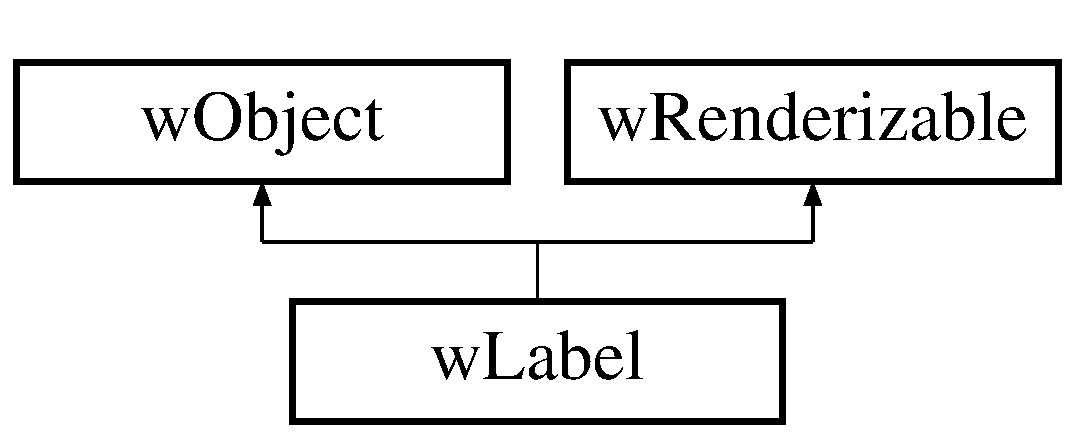
\includegraphics[height=2.000000cm]{classwLabel}
\end{center}
\end{figure}
\subsection*{Public Member Functions}
\begin{DoxyCompactItemize}
\item 
\hypertarget{classwLabel_a9cfc72c52cd114f7a6c2f8cbf3342ea1}{
{\bfseries \_\-\_\-construct} (\$name=null, \$parent, \$label, \$addPrefix=true)}
\label{classwLabel_a9cfc72c52cd114f7a6c2f8cbf3342ea1}

\item 
\hypertarget{classwLabel_a4af583bea5a3d8bbbd5c29e48b03a092}{
{\bfseries render} ()}
\label{classwLabel_a4af583bea5a3d8bbbd5c29e48b03a092}

\item 
\hypertarget{classwLabel_aeaece3629b7f812f32388e87b451cf82}{
{\bfseries \_\-setDefaults} ()}
\label{classwLabel_aeaece3629b7f812f32388e87b451cf82}

\end{DoxyCompactItemize}
\subsection*{Public Attributes}
\begin{DoxyCompactItemize}
\item 
\hypertarget{classwLabel_af2ea881445d2810ecd329cfe3622117c}{
{\bfseries \$label} = ''}
\label{classwLabel_af2ea881445d2810ecd329cfe3622117c}

\end{DoxyCompactItemize}


\subsection{Detailed Description}


Definition at line 3 of file wLabel.php.



The documentation for this class was generated from the following file:\begin{DoxyCompactItemize}
\item 
wLabel.php\end{DoxyCompactItemize}

\hypertarget{classwLayout}{
\section{wLayout Class Reference}
\label{classwLayout}\index{wLayout@{wLayout}}
}
Inheritance diagram for wLayout:\begin{figure}[H]
\begin{center}
\leavevmode
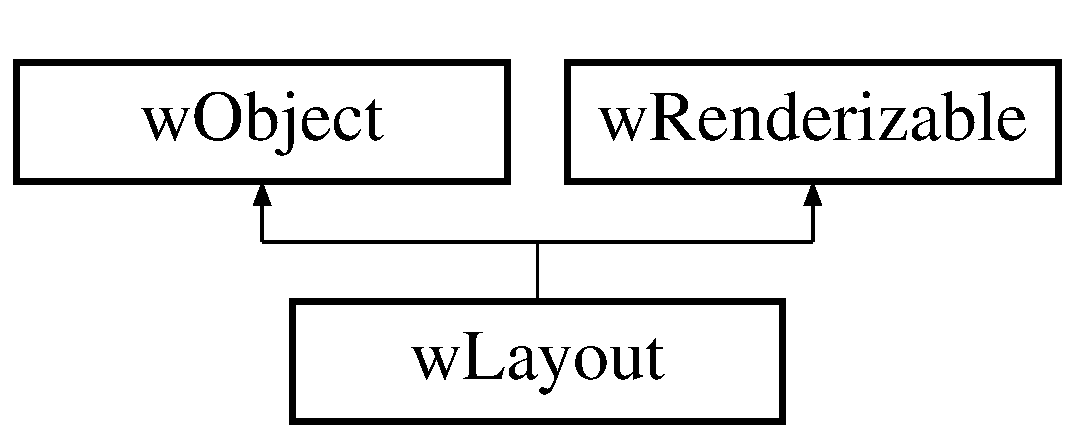
\includegraphics[height=2.000000cm]{classwLayout}
\end{center}
\end{figure}
\subsection*{Public Member Functions}
\begin{DoxyCompactItemize}
\item 
\hypertarget{classwLayout_a4b4fc51c9a01962fb39dc592cf74e6ba}{
{\bfseries \_\-\_\-construct} (\$name=null, \&\$parent)}
\label{classwLayout_a4b4fc51c9a01962fb39dc592cf74e6ba}

\item 
\hypertarget{classwLayout_a1c6a3599d1a330751b9783fc80c46348}{
{\bfseries render} ()}
\label{classwLayout_a1c6a3599d1a330751b9783fc80c46348}

\item 
\hypertarget{classwLayout_a8709289f21a12d7e5ac56ff100bf819b}{
{\bfseries setVertical} ()}
\label{classwLayout_a8709289f21a12d7e5ac56ff100bf819b}

\item 
\hypertarget{classwLayout_ac41d433795bb46a3510b11decab6d05b}{
{\bfseries setHorizontal} ()}
\label{classwLayout_ac41d433795bb46a3510b11decab6d05b}

\item 
\hypertarget{classwLayout_a4ca5e81203648719bfe77f4934f7ada0}{
{\bfseries \_\-setDefaults} ()}
\label{classwLayout_a4ca5e81203648719bfe77f4934f7ada0}

\end{DoxyCompactItemize}
\subsection*{Public Attributes}
\begin{DoxyCompactItemize}
\item 
\hypertarget{classwLayout_a5d4af8f9bc8eb86e8eea8ca5b6a83510}{
{\bfseries \$name} = \char`\"{}\char`\"{}}
\label{classwLayout_a5d4af8f9bc8eb86e8eea8ca5b6a83510}

\item 
\hypertarget{classwLayout_aea829d2f9e128a6fed14a9066784c02e}{
{\bfseries \$type} = 0}
\label{classwLayout_aea829d2f9e128a6fed14a9066784c02e}

\item 
\hypertarget{classwLayout_acb03f54f9326d0086dd0ad0dd35f4754}{
{\bfseries \$fixedSizes} = array()}
\label{classwLayout_acb03f54f9326d0086dd0ad0dd35f4754}

\end{DoxyCompactItemize}


\subsection{Detailed Description}


Definition at line 3 of file wLayout.php.



The documentation for this class was generated from the following file:\begin{DoxyCompactItemize}
\item 
wLayout.php\end{DoxyCompactItemize}

\hypertarget{classwListBox}{
\section{wListBox Class Reference}
\label{classwListBox}\index{wListBox@{wListBox}}
}
Inheritance diagram for wListBox:\begin{figure}[H]
\begin{center}
\leavevmode
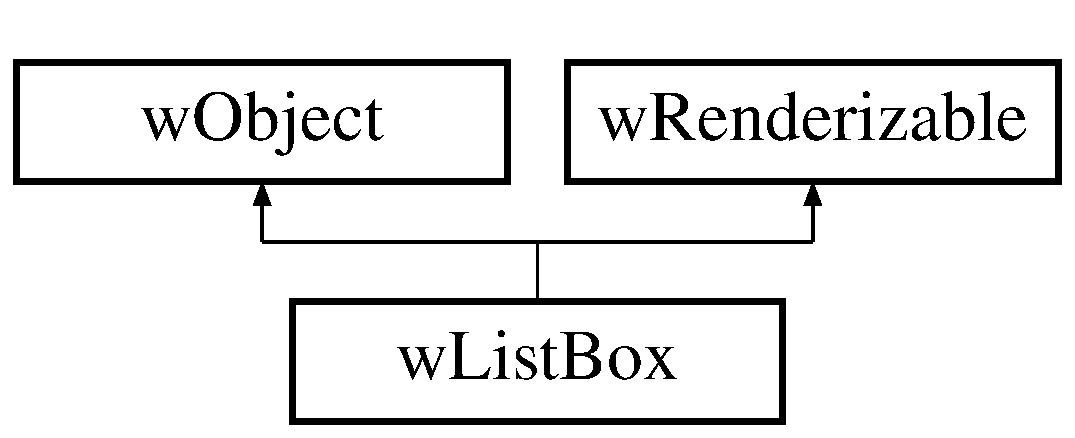
\includegraphics[height=2.000000cm]{classwListBox}
\end{center}
\end{figure}
\subsection*{Public Member Functions}
\begin{DoxyCompactItemize}
\item 
\hypertarget{classwListBox_a83b4f49e769483f784eb0e49da8f8135}{
{\bfseries \_\-\_\-construct} (\$name=null, \&\$parent, \$addPrefix=true)}
\label{classwListBox_a83b4f49e769483f784eb0e49da8f8135}

\item 
\hypertarget{classwListBox_af57c322706fb96114554dca85364e42f}{
{\bfseries render} ()}
\label{classwListBox_af57c322706fb96114554dca85364e42f}

\item 
\hypertarget{classwListBox_a5e64d56c76c0c82b3c974963f794d172}{
{\bfseries \_\-setDefaults} ()}
\label{classwListBox_a5e64d56c76c0c82b3c974963f794d172}

\item 
\hypertarget{classwListBox_a77fed9be31a93e528b9d9938abe266e8}{
{\bfseries setDataModel} (\$data)}
\label{classwListBox_a77fed9be31a93e528b9d9938abe266e8}

\item 
\hypertarget{classwListBox_a2413f57ed79bea737d3721abe54a3ffb}{
{\bfseries setSelectedIndex} (\$i)}
\label{classwListBox_a2413f57ed79bea737d3721abe54a3ffb}

\end{DoxyCompactItemize}
\subsection*{Public Attributes}
\begin{DoxyCompactItemize}
\item 
\hypertarget{classwListBox_a9abe7f2a9cbb9bc2789c36c6d6e5c9a2}{
{\bfseries \$name} = \char`\"{}\char`\"{}}
\label{classwListBox_a9abe7f2a9cbb9bc2789c36c6d6e5c9a2}

\item 
\hypertarget{classwListBox_a8284fd6edf5490e1a8d78b129c78dfdd}{
{\bfseries \$value} = \char`\"{}\char`\"{}}
\label{classwListBox_a8284fd6edf5490e1a8d78b129c78dfdd}

\item 
\hypertarget{classwListBox_aa6a0ca9020f7542312fb5eb4cd30370c}{
{\bfseries \$dataModel} = array()}
\label{classwListBox_aa6a0ca9020f7542312fb5eb4cd30370c}

\item 
\hypertarget{classwListBox_a4891812ac40824070b7394f794ca3534}{
{\bfseries \$moreHTMLproperties} = \char`\"{}\char`\"{}}
\label{classwListBox_a4891812ac40824070b7394f794ca3534}

\end{DoxyCompactItemize}


\subsection{Detailed Description}


Definition at line 3 of file wListBox.php.



The documentation for this class was generated from the following file:\begin{DoxyCompactItemize}
\item 
wListBox.php\end{DoxyCompactItemize}

\hypertarget{classwMutableLabel}{
\section{wMutableLabel Class Reference}
\label{classwMutableLabel}\index{wMutableLabel@{wMutableLabel}}
}
Inheritance diagram for wMutableLabel:\begin{figure}[H]
\begin{center}
\leavevmode
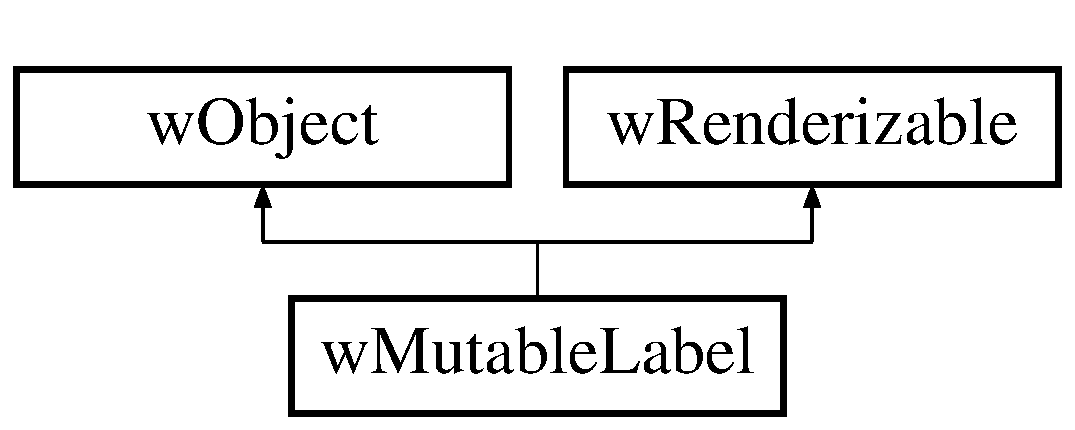
\includegraphics[height=2.000000cm]{classwMutableLabel}
\end{center}
\end{figure}
\subsection*{Public Member Functions}
\begin{DoxyCompactItemize}
\item 
\hypertarget{classwMutableLabel_aeb1dc8a750435ed494315db68beb1efa}{
{\bfseries \_\-\_\-construct} (\$name=null, \&\$parent, \$label)}
\label{classwMutableLabel_aeb1dc8a750435ed494315db68beb1efa}

\item 
\hypertarget{classwMutableLabel_a31bc6b7bddf6c1c7f3d01bb4d2577904}{
{\bfseries render} ()}
\label{classwMutableLabel_a31bc6b7bddf6c1c7f3d01bb4d2577904}

\item 
\hypertarget{classwMutableLabel_aa8e0a3bdbce29bc38208b6a2a564759a}{
{\bfseries \_\-setDefaults} ()}
\label{classwMutableLabel_aa8e0a3bdbce29bc38208b6a2a564759a}

\item 
\hypertarget{classwMutableLabel_a01f3ee9991b1e0d31530dc52dbb6c87a}{
{\bfseries setSelectedValue} (\$data)}
\label{classwMutableLabel_a01f3ee9991b1e0d31530dc52dbb6c87a}

\end{DoxyCompactItemize}
\subsection*{Public Attributes}
\begin{DoxyCompactItemize}
\item 
\hypertarget{classwMutableLabel_af2fc02b9061095455dddb112ec640d8e}{
{\bfseries \$name} = \char`\"{}\char`\"{}}
\label{classwMutableLabel_af2fc02b9061095455dddb112ec640d8e}

\item 
\hypertarget{classwMutableLabel_aafbc3b73949bbe0b2e37748e7dab0c44}{
{\bfseries \$value} = \char`\"{}\char`\"{}}
\label{classwMutableLabel_aafbc3b73949bbe0b2e37748e7dab0c44}

\end{DoxyCompactItemize}


\subsection{Detailed Description}


Definition at line 3 of file wMutableLabel.php.



The documentation for this class was generated from the following file:\begin{DoxyCompactItemize}
\item 
wMutableLabel.php\end{DoxyCompactItemize}

\hypertarget{classwObject}{
\section{wObject Class Reference}
\label{classwObject}\index{wObject@{wObject}}
}
Inheritance diagram for wObject:\begin{figure}[H]
\begin{center}
\leavevmode
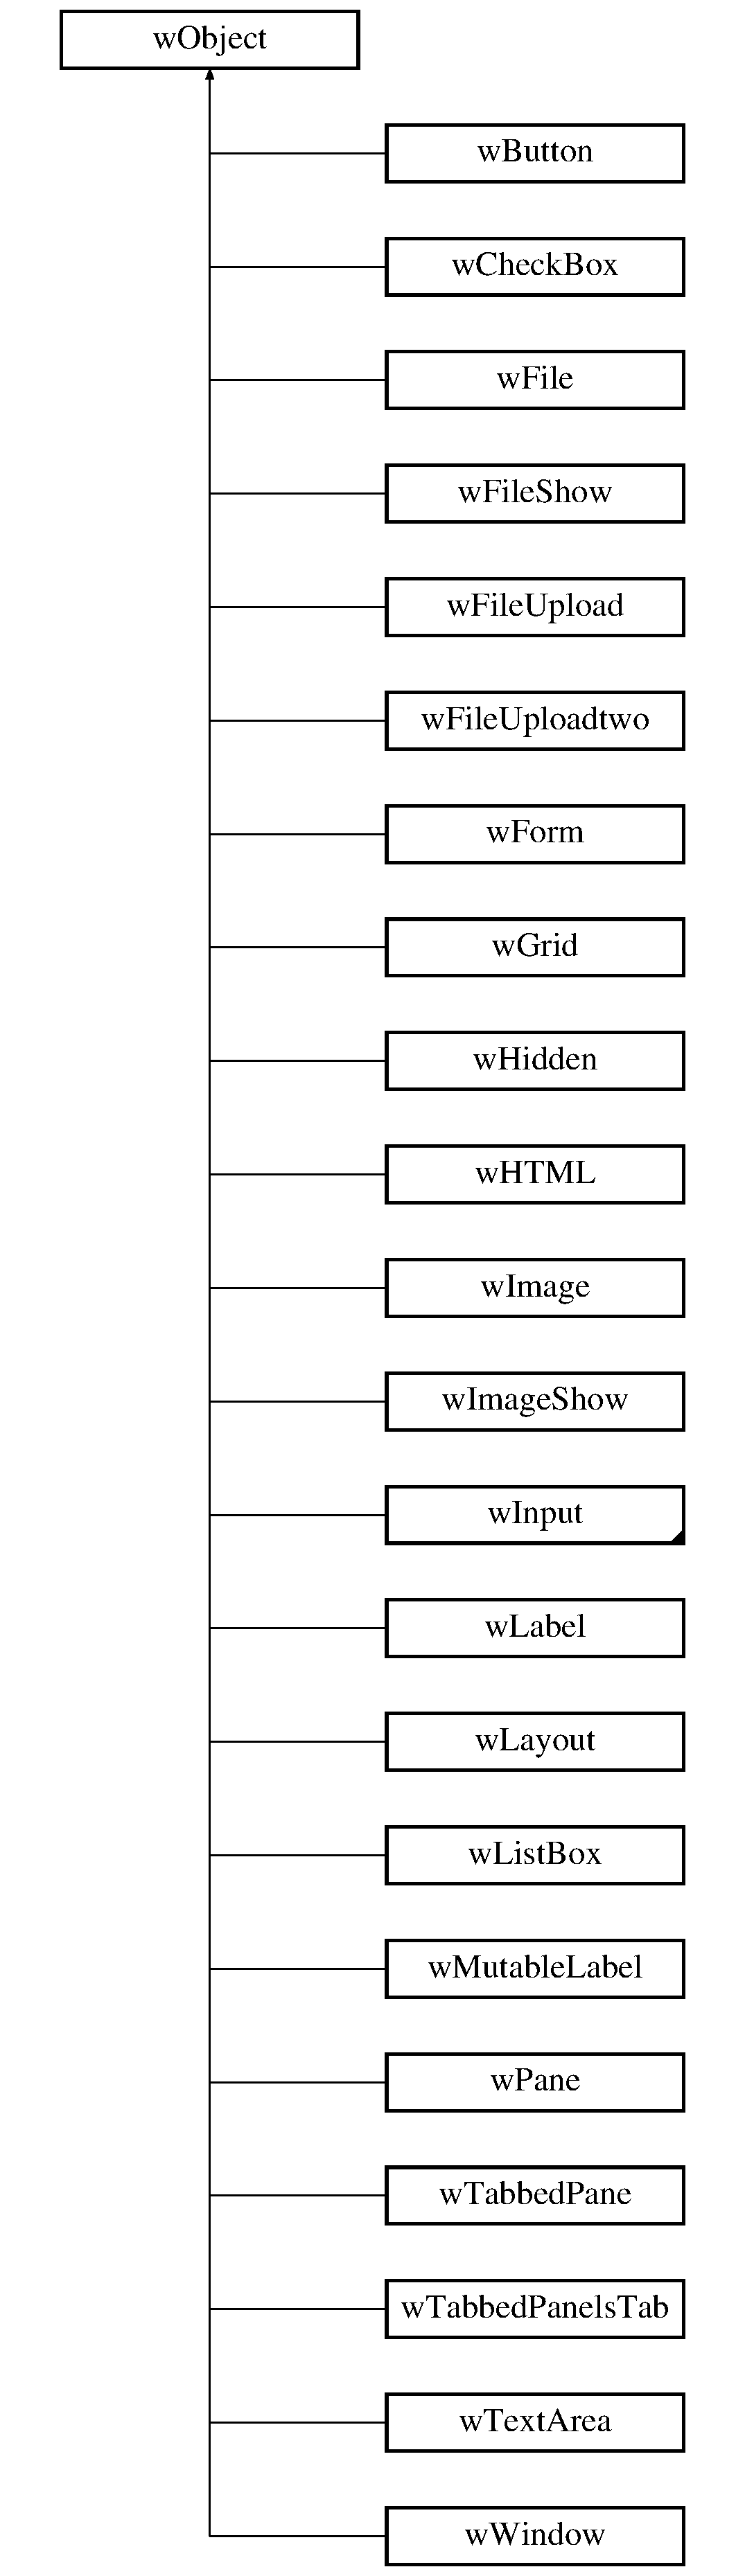
\includegraphics[height=12.000000cm]{classwObject}
\end{center}
\end{figure}
\subsection*{Public Member Functions}
\begin{DoxyCompactItemize}
\item 
\hypertarget{classwObject_a731a6cc6edc0a637da1d0578af14882e}{
{\bfseries \_\-\_\-construct} (\$name=null, \&\$parent=null)}
\label{classwObject_a731a6cc6edc0a637da1d0578af14882e}

\item 
\hypertarget{classwObject_a760d41e6c19257d292817b37c4920500}{
{\bfseries setCSS} (\$value, \$data)}
\label{classwObject_a760d41e6c19257d292817b37c4920500}

\item 
\hypertarget{classwObject_aaef0eb3d21c462c6028a24b956ffcd2f}{
{\bfseries add} (\&\$object)}
\label{classwObject_aaef0eb3d21c462c6028a24b956ffcd2f}

\item 
\hypertarget{classwObject_a047b73bd922b26d9567ebdafaefb36d5}{
{\bfseries addListener} (\$event, \$function, \$object=null)}
\label{classwObject_a047b73bd922b26d9567ebdafaefb36d5}

\end{DoxyCompactItemize}
\subsection*{Static Public Member Functions}
\begin{DoxyCompactItemize}
\item 
\hypertarget{classwObject_accbeaa3b6f4b463074d22e38277ff5be}{
static {\bfseries actionPerformed} (\$id, \$event)}
\label{classwObject_accbeaa3b6f4b463074d22e38277ff5be}

\end{DoxyCompactItemize}
\subsection*{Public Attributes}
\begin{DoxyCompactItemize}
\item 
\hypertarget{classwObject_a8be6afc58b52e1487a52b32da887205d}{
{\bfseries \$wChildren} = array()}
\label{classwObject_a8be6afc58b52e1487a52b32da887205d}

\item 
\hypertarget{classwObject_a564cf9353174fd8a29c6c43c98856669}{
{\bfseries \$wParent} = null}
\label{classwObject_a564cf9353174fd8a29c6c43c98856669}

\item 
\hypertarget{classwObject_af0838da9480973fe3ed12a541c4470ba}{
{\bfseries \$Listener} = array()}
\label{classwObject_af0838da9480973fe3ed12a541c4470ba}

\item 
\hypertarget{classwObject_ac77a081b86a9e364c8525ffa3da47b17}{
{\bfseries \$ListenerAux} = array()}
\label{classwObject_ac77a081b86a9e364c8525ffa3da47b17}

\item 
\hypertarget{classwObject_aa61efda77d012662d267f65e7ec0e434}{
{\bfseries \$id}}
\label{classwObject_aa61efda77d012662d267f65e7ec0e434}

\item 
\hypertarget{classwObject_abaf4a7af4e5ba939c294eb30c859da83}{
{\bfseries \$cssStyle} = ''}
\label{classwObject_abaf4a7af4e5ba939c294eb30c859da83}

\item 
\hypertarget{classwObject_afe7fc5f276159a917c3964ff1c9ae26c}{
{\bfseries \$staticCSS} = array()}
\label{classwObject_afe7fc5f276159a917c3964ff1c9ae26c}

\end{DoxyCompactItemize}


\subsection{Detailed Description}


Definition at line 4 of file wObject.php.



The documentation for this class was generated from the following file:\begin{DoxyCompactItemize}
\item 
wObject.php\end{DoxyCompactItemize}

\hypertarget{classwPane}{
\section{wPane Class Reference}
\label{classwPane}\index{wPane@{wPane}}
}
Inheritance diagram for wPane:\begin{figure}[H]
\begin{center}
\leavevmode
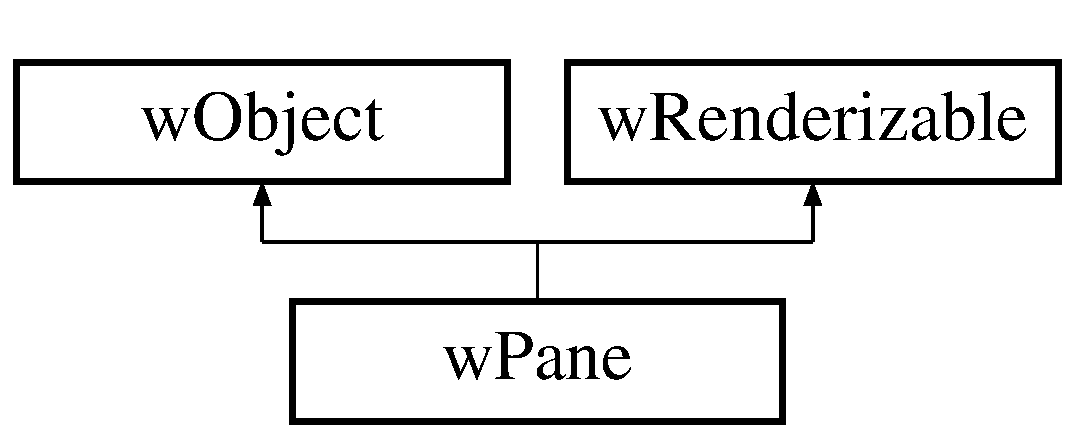
\includegraphics[height=2.000000cm]{classwPane}
\end{center}
\end{figure}
\subsection*{Public Member Functions}
\begin{DoxyCompactItemize}
\item 
\hypertarget{classwPane_af29a9a02589ce446d95b6db723513c4f}{
{\bfseries \_\-\_\-construct} (\$name=null, \&\$parent)}
\label{classwPane_af29a9a02589ce446d95b6db723513c4f}

\item 
\hypertarget{classwPane_a47d4d1cdd559921d86edc76a04772c56}{
{\bfseries render} ()}
\label{classwPane_a47d4d1cdd559921d86edc76a04772c56}

\item 
\hypertarget{classwPane_aa17d6c28641cadc85f68fdc94f7e328d}{
{\bfseries setVertical} ()}
\label{classwPane_aa17d6c28641cadc85f68fdc94f7e328d}

\item 
\hypertarget{classwPane_a4a1147f653f59751d095c9741f984381}{
{\bfseries setHorizontal} ()}
\label{classwPane_a4a1147f653f59751d095c9741f984381}

\item 
\hypertarget{classwPane_a62b27b879a9ed0a313ffcb12be9cefb1}{
{\bfseries \_\-setDefaults} ()}
\label{classwPane_a62b27b879a9ed0a313ffcb12be9cefb1}

\end{DoxyCompactItemize}
\subsection*{Public Attributes}
\begin{DoxyCompactItemize}
\item 
\hypertarget{classwPane_a0d588bc913c35cd31458ed1aaa665952}{
{\bfseries \$name} = \char`\"{}\char`\"{}}
\label{classwPane_a0d588bc913c35cd31458ed1aaa665952}

\item 
\hypertarget{classwPane_a451ef86704751fb05e90ccc4b5b4866b}{
{\bfseries \$type} = 0}
\label{classwPane_a451ef86704751fb05e90ccc4b5b4866b}

\item 
\hypertarget{classwPane_afda42b6f23d97d884842397df9344363}{
{\bfseries \$visibility} = \char`\"{}visible\char`\"{}}
\label{classwPane_afda42b6f23d97d884842397df9344363}

\end{DoxyCompactItemize}


\subsection{Detailed Description}


Definition at line 3 of file wPane.php.



The documentation for this class was generated from the following file:\begin{DoxyCompactItemize}
\item 
wPane.php\end{DoxyCompactItemize}

\hypertarget{interfacewRenderizable}{
\section{wRenderizable Interface Reference}
\label{interfacewRenderizable}\index{wRenderizable@{wRenderizable}}
}
Inheritance diagram for wRenderizable:\begin{figure}[H]
\begin{center}
\leavevmode
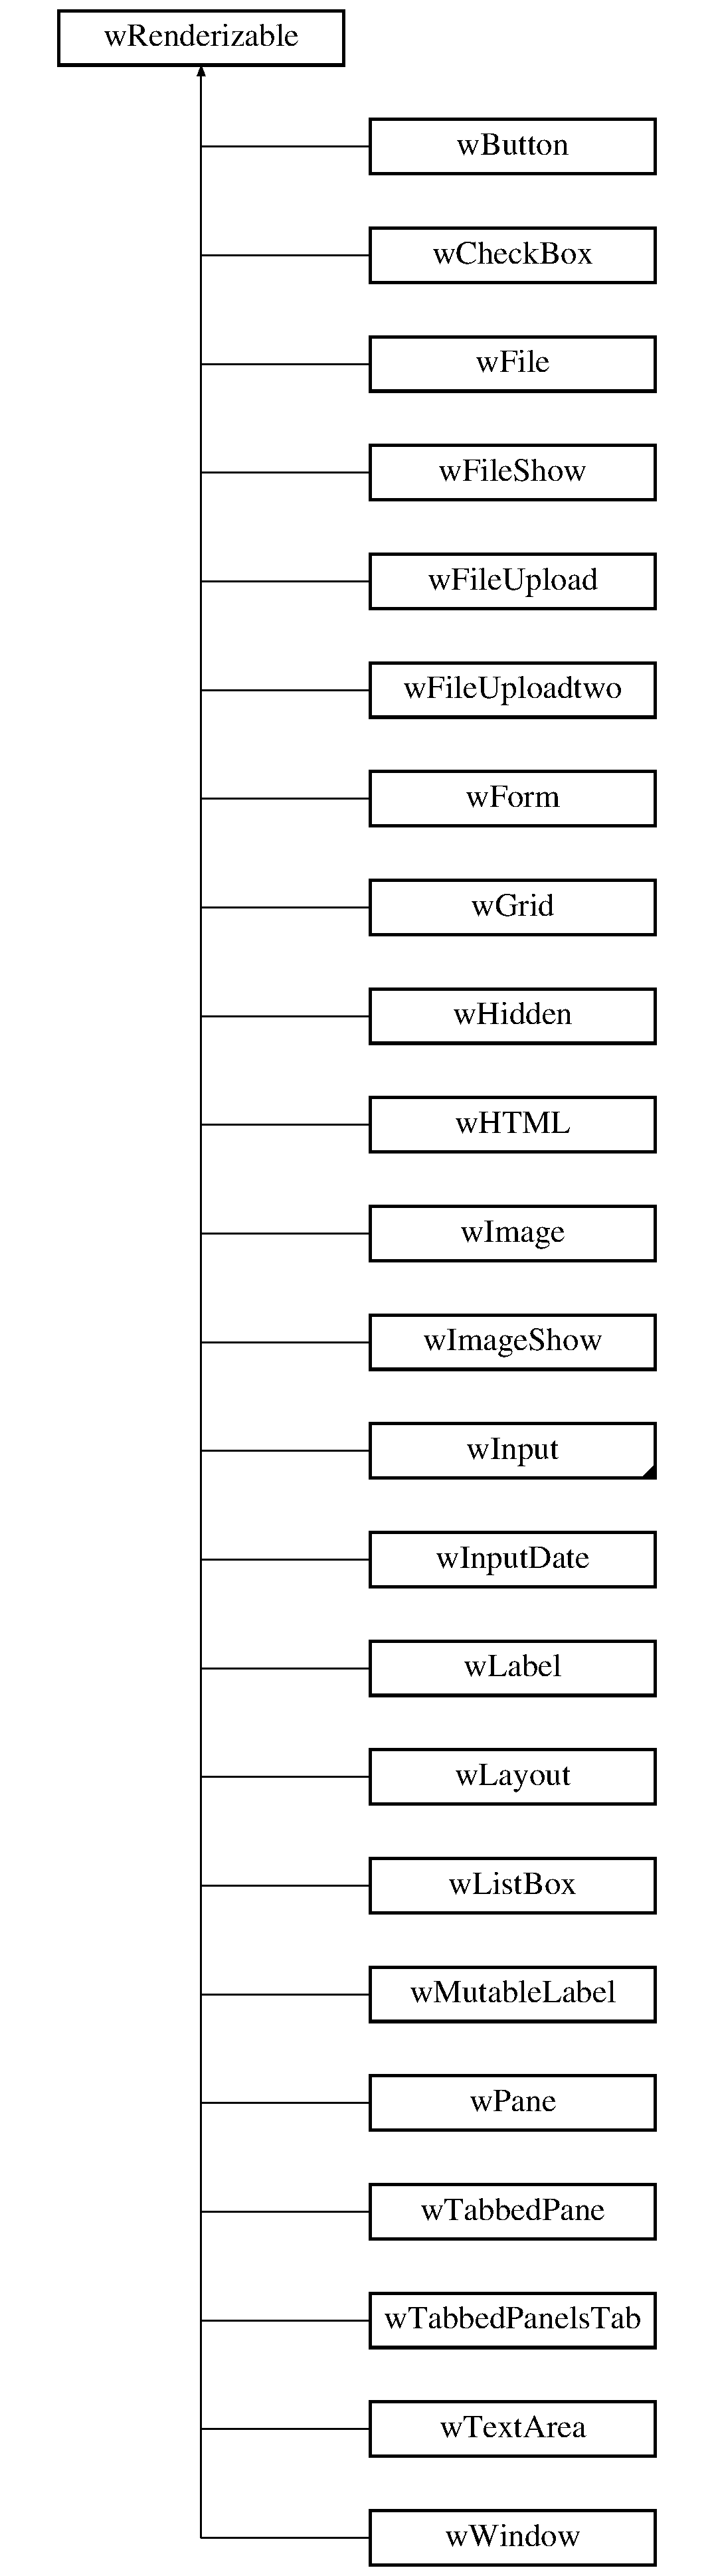
\includegraphics[height=12.000000cm]{interfacewRenderizable}
\end{center}
\end{figure}
\subsection*{Public Member Functions}
\begin{DoxyCompactItemize}
\item 
\hypertarget{interfacewRenderizable_a53efe86d5a3106fbd10a90e3ccac4335}{
{\bfseries Render} ()}
\label{interfacewRenderizable_a53efe86d5a3106fbd10a90e3ccac4335}

\end{DoxyCompactItemize}


\subsection{Detailed Description}


Definition at line 3 of file wUI.php.



The documentation for this interface was generated from the following file:\begin{DoxyCompactItemize}
\item 
wUI.php\end{DoxyCompactItemize}

\hypertarget{classwTabbedPane}{
\section{wTabbedPane Class Reference}
\label{classwTabbedPane}\index{wTabbedPane@{wTabbedPane}}
}
Inheritance diagram for wTabbedPane:\begin{figure}[H]
\begin{center}
\leavevmode
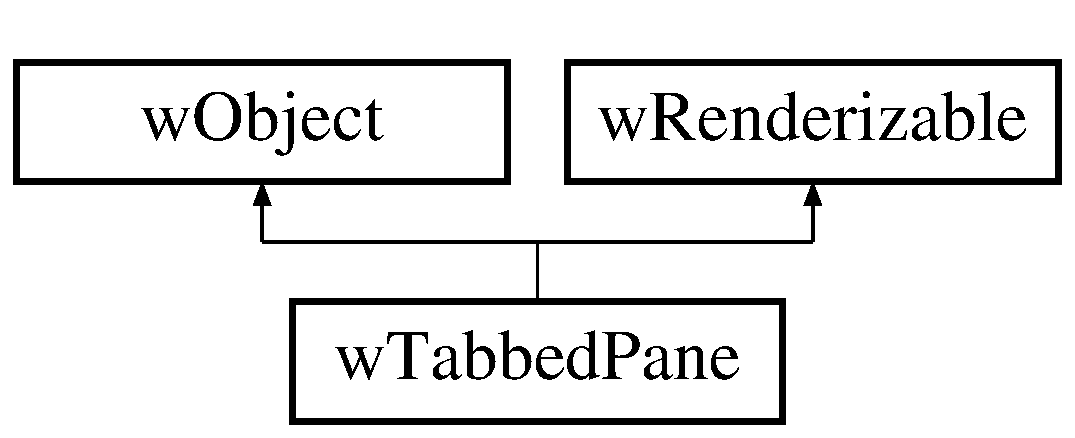
\includegraphics[height=2.000000cm]{classwTabbedPane}
\end{center}
\end{figure}
\subsection*{Public Member Functions}
\begin{DoxyCompactItemize}
\item 
\hypertarget{classwTabbedPane_ae805392b9455756b4e31802e1748c52a}{
{\bfseries setHTML} (\$HTML)}
\label{classwTabbedPane_ae805392b9455756b4e31802e1748c52a}

\item 
\hypertarget{classwTabbedPane_a57255405a9c4e444ac2934d0fb22af41}{
{\bfseries render} ()}
\label{classwTabbedPane_a57255405a9c4e444ac2934d0fb22af41}

\item 
\hypertarget{classwTabbedPane_a7ef6330ae936bce535ffb1960086c099}{
{\bfseries \_\-setDefaults} ()}
\label{classwTabbedPane_a7ef6330ae936bce535ffb1960086c099}

\end{DoxyCompactItemize}
\subsection*{Public Attributes}
\begin{DoxyCompactItemize}
\item 
\hypertarget{classwTabbedPane_a94c1683b7caee875db7b3f43144efa31}{
{\bfseries \$content}}
\label{classwTabbedPane_a94c1683b7caee875db7b3f43144efa31}

\item 
\hypertarget{classwTabbedPane_af6939118bf38c182ad97afc5371d7bb2}{
{\bfseries \$name} = \char`\"{}\char`\"{}}
\label{classwTabbedPane_af6939118bf38c182ad97afc5371d7bb2}

\item 
\hypertarget{classwTabbedPane_a30950db583a10ecda9cfccb92fb2d4fc}{
{\bfseries \$label} = \char`\"{}\char`\"{}}
\label{classwTabbedPane_a30950db583a10ecda9cfccb92fb2d4fc}

\end{DoxyCompactItemize}


\subsection{Detailed Description}


Definition at line 3 of file wTabbedPane.php.



The documentation for this class was generated from the following file:\begin{DoxyCompactItemize}
\item 
wTabbedPane.php\end{DoxyCompactItemize}

\hypertarget{classwTabbedPanelsTab}{
\section{wTabbedPanelsTab Class Reference}
\label{classwTabbedPanelsTab}\index{wTabbedPanelsTab@{wTabbedPanelsTab}}
}
Inheritance diagram for wTabbedPanelsTab:\begin{figure}[H]
\begin{center}
\leavevmode
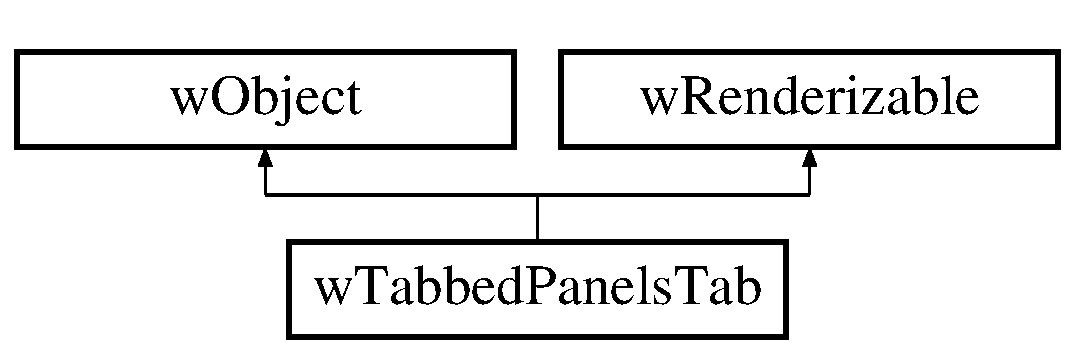
\includegraphics[height=2.000000cm]{classwTabbedPanelsTab}
\end{center}
\end{figure}
\subsection*{Public Member Functions}
\begin{DoxyCompactItemize}
\item 
\hypertarget{classwTabbedPanelsTab_a7e95589bca465bedb929ddfa5aba4772}{
{\bfseries setHTML} (\$HTML)}
\label{classwTabbedPanelsTab_a7e95589bca465bedb929ddfa5aba4772}

\item 
\hypertarget{classwTabbedPanelsTab_ab7a26547f4986c40b88db043d943ec66}{
{\bfseries render} ()}
\label{classwTabbedPanelsTab_ab7a26547f4986c40b88db043d943ec66}

\item 
\hypertarget{classwTabbedPanelsTab_a79db8f792fab6f0c69a765ede0877faa}{
{\bfseries \_\-setDefaults} ()}
\label{classwTabbedPanelsTab_a79db8f792fab6f0c69a765ede0877faa}

\end{DoxyCompactItemize}
\subsection*{Public Attributes}
\begin{DoxyCompactItemize}
\item 
\hypertarget{classwTabbedPanelsTab_a79ea3eb43c3c3d023e0031455c497ed6}{
{\bfseries \$content}}
\label{classwTabbedPanelsTab_a79ea3eb43c3c3d023e0031455c497ed6}

\item 
\hypertarget{classwTabbedPanelsTab_afdcbdfc74164d6c6eeccb705c1287a28}{
{\bfseries \$name} = \char`\"{}\char`\"{}}
\label{classwTabbedPanelsTab_afdcbdfc74164d6c6eeccb705c1287a28}

\item 
\hypertarget{classwTabbedPanelsTab_a8e7f16b7d7acc993ba1d1d2dd738e43d}{
{\bfseries \$label} = \char`\"{}\char`\"{}}
\label{classwTabbedPanelsTab_a8e7f16b7d7acc993ba1d1d2dd738e43d}

\end{DoxyCompactItemize}


\subsection{Detailed Description}


Definition at line 3 of file wTabbedPanelsTab.php.



The documentation for this class was generated from the following file:\begin{DoxyCompactItemize}
\item 
wTabbedPanelsTab.php\end{DoxyCompactItemize}

\hypertarget{classwTextArea}{
\section{wTextArea Class Reference}
\label{classwTextArea}\index{wTextArea@{wTextArea}}
}
Inheritance diagram for wTextArea:\begin{figure}[H]
\begin{center}
\leavevmode
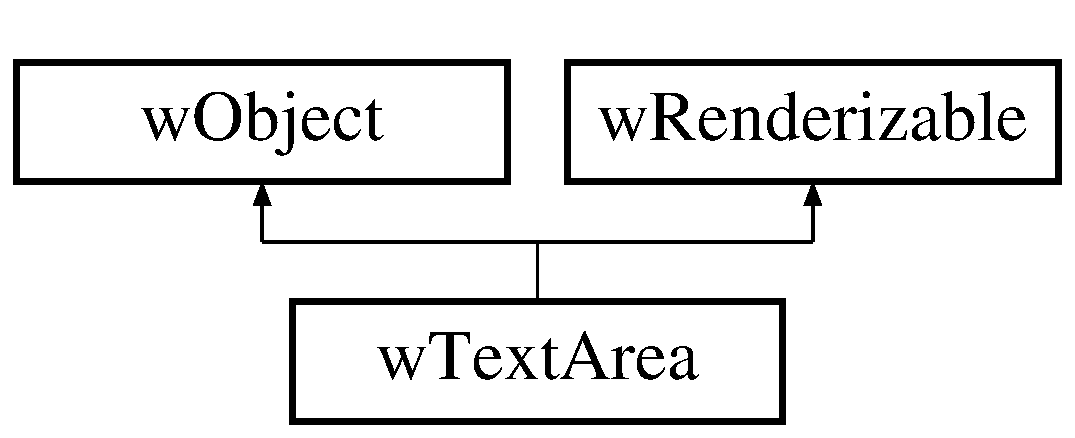
\includegraphics[height=2.000000cm]{classwTextArea}
\end{center}
\end{figure}
\subsection*{Public Member Functions}
\begin{DoxyCompactItemize}
\item 
\hypertarget{classwTextArea_ac2bb1f60b5a304b790e972637bd102c0}{
{\bfseries \_\-\_\-construct} (\$name=null, \&\$parent, \$addPrefix=true)}
\label{classwTextArea_ac2bb1f60b5a304b790e972637bd102c0}

\item 
\hypertarget{classwTextArea_ab09b8b2d77923bbb1ce7d043e0e34142}{
{\bfseries render} ()}
\label{classwTextArea_ab09b8b2d77923bbb1ce7d043e0e34142}

\item 
\hypertarget{classwTextArea_a5c3f2a4563ab1bd286a2a90889eecb2e}{
{\bfseries \_\-setDefaults} ()}
\label{classwTextArea_a5c3f2a4563ab1bd286a2a90889eecb2e}

\item 
\hypertarget{classwTextArea_afca9ef9f3e02351c34cf4c48c0daf123}{
{\bfseries setSelectedValue} (\$data)}
\label{classwTextArea_afca9ef9f3e02351c34cf4c48c0daf123}

\end{DoxyCompactItemize}
\subsection*{Public Attributes}
\begin{DoxyCompactItemize}
\item 
\hypertarget{classwTextArea_a32a593b28a7dfaadf235b7a609ecccdb}{
{\bfseries \$name} = \char`\"{}\char`\"{}}
\label{classwTextArea_a32a593b28a7dfaadf235b7a609ecccdb}

\item 
\hypertarget{classwTextArea_a422280ac1718e5e38f582a6892e9528a}{
{\bfseries \$value} = \char`\"{}\char`\"{}}
\label{classwTextArea_a422280ac1718e5e38f582a6892e9528a}

\end{DoxyCompactItemize}


\subsection{Detailed Description}


Definition at line 3 of file wTextArea.php.



The documentation for this class was generated from the following file:\begin{DoxyCompactItemize}
\item 
wTextArea.php\end{DoxyCompactItemize}

\hypertarget{classwWindow}{
\section{wWindow Class Reference}
\label{classwWindow}\index{wWindow@{wWindow}}
}
Inheritance diagram for wWindow:\begin{figure}[H]
\begin{center}
\leavevmode
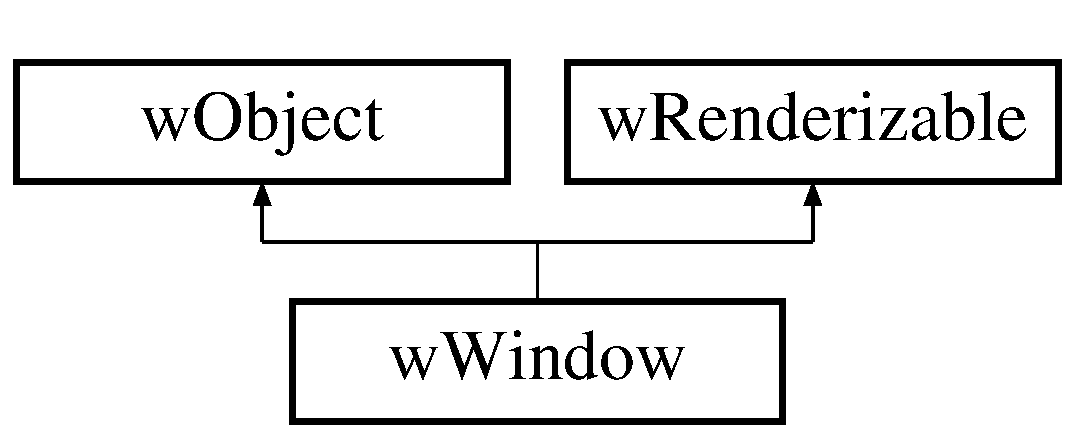
\includegraphics[height=2.000000cm]{classwWindow}
\end{center}
\end{figure}
\subsection*{Public Member Functions}
\begin{DoxyCompactItemize}
\item 
\hypertarget{classwWindow_a86d32d44e921532279470c74f25cb192}{
{\bfseries \_\-\_\-construct} (\$name=null, \&\$parent=null, \$addPrefix=true)}
\label{classwWindow_a86d32d44e921532279470c74f25cb192}

\item 
\hypertarget{classwWindow_ae571fa5f25b5a200559152153fd0414d}{
{\bfseries render} ()}
\label{classwWindow_ae571fa5f25b5a200559152153fd0414d}

\item 
\hypertarget{classwWindow_a066bca3555dce86d7f9d18fbe3d7fc4f}{
{\bfseries \_\-setDefaults} ()}
\label{classwWindow_a066bca3555dce86d7f9d18fbe3d7fc4f}

\end{DoxyCompactItemize}
\subsection*{Public Attributes}
\begin{DoxyCompactItemize}
\item 
\hypertarget{classwWindow_a5b70c9b41159c1e8ddef1121b0c75d7d}{
{\bfseries \$name} = \char`\"{}\char`\"{}}
\label{classwWindow_a5b70c9b41159c1e8ddef1121b0c75d7d}

\item 
\hypertarget{classwWindow_a3fcc1893184df1d10cbf1c99cdd0153b}{
{\bfseries \$title} = \char`\"{}\char`\"{}}
\label{classwWindow_a3fcc1893184df1d10cbf1c99cdd0153b}

\item 
\hypertarget{classwWindow_aa19fc63dfefc91b456b74f0253806085}{
{\bfseries \$type} = 0}
\label{classwWindow_aa19fc63dfefc91b456b74f0253806085}

\end{DoxyCompactItemize}


\subsection{Detailed Description}


Definition at line 3 of file wWindow.php.



The documentation for this class was generated from the following file:\begin{DoxyCompactItemize}
\item 
wWindow.php\end{DoxyCompactItemize}

\printindex
\end{document}
